\documentclass{article}
\nonstopmode % prevent interactive halt on errors

% NeurIPS 2025 format package — style strictly from Styles/ folder
\usepackage[final,main]{Styles/neurips_2025}

\usepackage[utf8]{inputenc} % allow utf-8 input
\usepackage[T5]{fontenc}    % use T5 for Vietnamese
\usepackage[utf8]{vietnam}  % Vietnamese support
\usepackage{hyperref}       % hyperlinks
\usepackage{url}            % simple URL typesetting
\usepackage{booktabs}       % professional-quality tables
\usepackage{amsfonts}       % blackboard math symbols
\usepackage{nicefrac}       % compact symbols for 1/2, etc.
\usepackage{microtype}      % microtypography
\usepackage{xcolor}         % colors
\usepackage{graphicx}       % images
\graphicspath{{datathon-2026-round-1/output/}} % default image search path
\usepackage{caption}
\usepackage{subcaption}
\usepackage{rotating}       % for sidewaysfigure

\title{BÁO CÁO PHÂN TÍCH: KEY INSIGHTS \& MÔ HÌNH DỰ BÁO DOANH THU}

\author{%
  Team 4Chickens \\
  VinTelligence Datathon 2026 \\
  \texttt{https://github.com/trmuba2502/VinUni_Datathon_4Chickens} \\
}

\begin{document}

\maketitle

\begin{abstract}
  \textbf{Tóm tắt nội dung}\\
  Báo cáo tập trung phân tích hành vi mua sắm, hiệu quả vận hành và hoạch định chiến lược kinh doanh dựa trên dữ liệu (Data-driven Insights) giai đoạn 2012-2022. Đặc biệt, báo cáo đề xuất một đường ống (pipeline) học máy dự báo doanh thu chuỗi thời gian cho giai đoạn 2023-2024. Pipeline này được thiết kế với cơ chế kiểm soát rò rỉ dữ liệu (data leakage) khắt khe, kết hợp ứng dụng SHAP (Explainable AI) để minh bạch hóa thuật toán, từ đó tối ưu phân bổ tồn kho và tối đa hóa biên lợi nhuận.
\end{abstract}

\section{Trực quan hoá và Phân tích Dữ liệu (EDA)}

Dựa trên việc trực quan hóa và chẩn đoán toàn diện cơ sở dữ liệu qua 18 Dashboard, chúng tôi tập trung bóc tách 4 khía cạnh trọng điểm. Các phân tích được đối chiếu xuyên suốt 4 cấp độ: Mô tả (Descriptive), Chẩn đoán (Diagnostic), Dự đoán (Predictive) và Đề xuất (Prescriptive) nhằm thiết lập các chiến lược hành động mang lại giá trị định lượng cao.

\subsection{Mô hình Hành vi Khách hàng \& Phân khúc (Customer Segmentation)}

\textbf{Insight 1.1: Trụ cột lợi nhuận "Everyday \& Balanced" (Độ tuổi 25-44)} \\
\textbf{Chẩn đoán:} Phân tích Heatmap (xem Hình \ref{fig:chart17}) chỉ ra phân khúc Everyday và Balanced ở tệp khách hàng trưởng thành (25-44 tuổi) đóng vai trò là động lực sinh lời chủ đạo, mang lại phần lớn tỷ trọng lợi nhuận cho toàn hệ thống. Ngược lại, các dòng sản phẩm ngách (All-weather, Premium) ghi nhận mức sinh lời vô cùng khiêm tốn (dưới 5 triệu VNĐ/nhóm tuổi). Dữ liệu phản ánh ý định mua sắm (purchase intent) của khách hàng tập trung mạnh vào tính ứng dụng và giá trị thực tiễn thay vì định vị thời trang cao cấp.
\\
\textbf{Đề xuất:} Cơ cấu lại dòng vốn R\&D bằng cách cắt giảm ngân sách phát triển của dòng Premium và All-weather. Tái định tuyến 75\% ngân sách R\&D (giai đoạn 1 \& 2) để nâng cấp trải nghiệm sản phẩm cho dòng Everyday (25-54 tuổi) và Balanced (25-44 tuổi). Về chiến lược Marketing, doanh nghiệp cần giới hạn chi phí tiếp thị đối với tệp phân khúc cao cấp, tập trung đẩy mạnh thông điệp "Thời trang ứng dụng hàng ngày" nhắm trực diện vào tệp khách hàng công sở.

\textbf{Insight 1.2: Cấu trúc "Sức mua theo Giới tính"} \\
\textbf{Chẩn đoán:} Tỷ trọng đóng góp lợi nhuận giữa Nam và Nữ đạt mức đối xứng 50-50 trên mọi nhóm tuổi. Dù vậy, đối với tệp khách hàng trên 35 tuổi của dòng Everyday, Nữ giới thể hiện tỷ lệ duy trì (retention rate) bền vững hơn. Trong khi đó, Nam giới cho thấy mức độ trung thành cao với các kiểu dáng quen thuộc nếu sản phẩm đáp ứng tiêu chuẩn chất lượng, giúp doanh nghiệp tiết kiệm đáng kể chi phí thu hút khách hàng mới (Customer Acquisition Cost - CAC).
\\
\textbf{Đề xuất:} Triển khai chiến lược truyền thông bao hàm giới tính (Gender-inclusive). Phát triển các gói sản phẩm kết hợp (Bundle/Combo dành cho gia đình hoặc cặp đôi) nhằm khai thác tối đa vị thế "người ra quyết định chi tiêu cuối cùng" của nhóm khách hàng Nữ.

\textbf{Insight 1.3: Hiệu suất Kênh thu hút khách hàng (Acquisition Channels)} \\
\textbf{Chẩn đoán:} Biểu đồ Bubble (xem Hình \ref{fig:chart7}) bộc lộ sự chênh lệch lớn trong hiệu suất của các phễu thu hút: Kênh tìm kiếm tự nhiên (Organic Search) là động lực tăng trưởng cốt lõi mang về 295 triệu VNĐ tổng lợi nhuận, vượt xa kênh Email (119 triệu VNĐ) và Referral (96 triệu VNĐ). Kênh Referral (Giới thiệu) mặc dù mang tính lan truyền cao nhưng lại ghi nhận tỷ lệ chuyển đổi thành tệp khách hàng sinh lời thấp nhất do hành vi lạm dụng chính sách ưu đãi (promotion abuse). Trái lại, lưu lượng từ Organic Search sở hữu mức độ sẵn lòng chi trả (Willingness to Pay) vượt trội.
\\
\textbf{Đề xuất:} Tinh giảm ngân sách tiếp thị từ kênh Referral. Chuyển dịch dòng vốn này để đầu tư chuyên sâu vào Tối ưu hóa công cụ tìm kiếm (SEO), Content Marketing và kiến trúc dữ liệu web nhằm duy trì vững chắc tệp khách hàng có biên lợi nhuận cao này.

\subsection{Hiệu quả Vận hành \& Quản trị Rủi ro Tài chính (Operations \& Risks)}

\textbf{Insight 2.1: Rủi ro từ Thanh toán Tiền mặt (COD) \& Sự phân tán của Trả góp 2 Kỳ} \\
\textbf{Chẩn đoán:} Phương thức thanh toán khi nhận hàng (COD) ghi nhận tỷ lệ hủy đơn (Cancellation Rate) xấp xỉ 16\%, cao gấp đôi mức trung bình 8\% của nhóm Thẻ tín dụng/Ví điện tử (xem Hình \ref{fig:chart10}). Hành vi đặt hàng thiếu ràng buộc tài chính trả trước đã trực tiếp làm gia tăng chi phí Logistics ngược (Reverse Logistics). Ở nhóm Trả góp 2 tháng (Installment-2), biên lợi nhuận gần như tiệm cận 0 kèm theo tỷ lệ hoàn trả cao kỷ lục (xem Hình \ref{fig:chart11}). Phân khúc này chủ yếu thu hút nhóm khách hàng có quyết định mua sắm ngẫu hứng, năng lực tài chính hạn chế và có tỷ lệ thay đổi ý định cao sau khi đặt hàng. Ngược lại, các gói thanh toán toàn bộ và trả góp 3 kỳ vẫn đang vận hành hiệu quả.
\\
\textbf{Đề xuất:} Quản trị rủi ro thanh toán COD: Thiết lập cơ chế kiểm soát bằng quy định thanh toán trước 20-30\% (hoặc thanh toán phí vận chuyển) đối với các đơn hàng có giá trị trên 500.000 VNĐ. Cung cấp quyền lợi trợ giá 5-10\% hoặc miễn phí vận chuyển nhằm điều hướng hành vi thanh toán sang Thẻ tín dụng/Ví điện tử. Tinh giản danh mục tài chính: Loại bỏ ngay lập tức tùy chọn Trả góp 2 kỳ, cấu trúc lại quy trình thanh toán chỉ giữ các gói trả thẳng hoặc trả góp 3 kỳ để thanh lọc chất lượng tín dụng khách hàng.

\textbf{Insight 2.2: Phân tích chênh lệch giữa Quy mô đơn hàng và Lợi nhuận (City Volume vs Profit)} \\
\textbf{Chẩn đoán:} Số lượng đơn hàng lớn tại một số đô thị không tỷ lệ thuận với dòng tiền thực tế doanh nghiệp nhận được. Gánh nặng chi phí vận chuyển hoặc hành vi tiêu dùng phụ thuộc nhiều vào các chương trình khuyến mãi đã tạo ra mức tăng trưởng về quy mô (volume) nhưng làm suy giảm biên lợi nhuận thực tế (margin).
\\
\textbf{Đề xuất:} Phân tầng thị trường địa lý thay vì áp dụng chính sách ưu đãi đồng nhất. Xây dựng chiến lược: "Tier 1: High Margin City" (Tập trung ngân sách quảng cáo cho hàng nguyên giá, chiến thuật bán chéo - cross-selling) và "Tier 2: High Volume - Low Margin City" (Thiết lập thành các điểm phân phối chiến lược để thanh lý hàng tồn đọng qua các gói sản phẩm kết hợp nhằm thu hồi vốn).

\subsection{Tác động Vĩ mô \& Phục hồi Phễu Chuyển Đổi (COVID-19 Recovery)}

\textbf{Insight 3.1: Đứt gãy Phễu Chuyển Đổi (Conversion Rate Collapse)} \\
\textbf{Chẩn đoán:} Dữ liệu lịch sử bộc lộ một sự đứt gãy cấu trúc nghiêm trọng (xem Hình \ref{fig:chart14}): Mặc dù lưu lượng truy cập (Sessions) đã phục hồi 100\% so với trước đại dịch, Lợi nhuận ròng (Net Profit) chỉ đạt mức 30\%. Tỷ lệ chuyển đổi (Conversion Rate) suy thoái nặng nề xuống mức 25-37\%. Khách hàng mang tâm lý thận trọng, chủ yếu duy trì hành vi tham khảo thông tin (window-shopping) thay vì tiến hành thanh toán. Tình trạng này cũng phản ánh thiết kế giao diện/trải nghiệm người dùng (UX/UI) tại bước thanh toán có thể đang tồn tại những điểm nghẽn (friction).
\\
\textbf{Đề xuất:} Tối ưu hóa Tỷ lệ Chuyển đổi (CRO): Tạm ngưng các chiến dịch quảng cáo diện rộng có hiệu suất thấp ở đầu phễu (Top-of-funnel Ads). Tập trung nguồn lực tái thiết kế trải nghiệm người dùng tại luồng thanh toán (Checkout flow). Tích hợp thêm các hệ thống nhắc nhở (như Exit-intent Popups cung cấp ưu đãi giới hạn thời gian) để kích thích quyết định mua hàng đối với nhóm khách hàng đang do dự.

\textbf{Insight 3.2: Hệ quả của chính sách siết chặt khuyến mãi} \\
\textbf{Chẩn đoán:} Phản ứng trước áp lực tỷ lệ hoàn trả cao năm 2015, doanh nghiệp đã thực thi chính sách thắt chặt mã giảm giá từ năm 2018. Khi bước sang giai đoạn phục hồi hậu đại dịch — thời điểm người tiêu dùng trở nên vô cùng nhạy cảm với sự biến động giá — việc hạn chế các chính sách kích cầu đã trở thành nguyên nhân trực tiếp làm kìm hãm đà phục hồi của Tỷ lệ chuyển đổi.
\\
\textbf{Đề xuất:} Tái cấu trúc danh mục khuyến mãi theo hướng linh hoạt và tối ưu chi phí. Thay vì giảm trừ trực tiếp trên giá niêm yết, doanh nghiệp nên ứng dụng các chiến thuật gia tăng giá trị như "Miễn phí giao hàng cho đơn từ 400.000 VNĐ" hoặc "Mua 3 tính tiền 2". Cấu trúc này vừa gia tăng giá trị trung bình trên mỗi đơn hàng (AOV), hỗ trợ giải phóng hàng tồn kho, vừa đáp ứng được nhu cầu tối ưu hóa chi phí của người tiêu dùng.

\subsection{Hoạch định Chuỗi Cung ứng \& Quản trị Tồn kho (Supply Chain)}

\textbf{Insight 4.1: Tính chu kỳ nội tuần của Tốc độ Thanh khoản} \\
\textbf{Chẩn đoán:} Phân tích dữ liệu bác bỏ giả định mua sắm tập trung vào cuối tuần, khẳng định Thứ 3, Thứ 4 và Thứ 5 mới là điểm rơi thanh khoản cao nhất (xem Hình \ref{fig:chart9}). Xét theo kích cỡ (Size), nhu cầu đối với size L và XL tăng trưởng đột biến vào Quý 4 (nhóm trang phục form rộng mùa lạnh, xem Hình \ref{fig:chartC}). Mô hình hoạch định size tĩnh (ví dụ tỷ lệ cố định 1S:2M:2L:1XL) được áp dụng dàn trải quanh năm đã trực tiếp gây ra trạng thái ứ đọng tồn kho (Overstock) tại một số mã sản phẩm, đồng thời đứt gãy chuỗi cung ứng (Stockout) ở các mã khác. Điều này cho thấy hệ thống lập kế hoạch mua hàng đang thiếu tính linh hoạt.
\\
\textbf{Đề xuất:} Tái định vị thời gian triển khai các chiến dịch ra mắt sản phẩm mới, Email Marketing và Push Notification sang khung giờ trưa Thứ 3 và Thứ 4 để tối đa hóa lưu lượng tiếp cận. Chấm dứt việc sử dụng tỷ lệ phân bổ size cố định trong quy trình hoạch định vật tư.

\textbf{Insight 4.2: Tối ưu hóa Kế hoạch Hoạt động và Kinh doanh (S\&OP Planning)} \\
\textbf{Chẩn đoán:} Tính mùa vụ có tác động vô cùng sâu sắc đến biên độ lợi nhuận của các Danh mục (Category - xem Hình \ref{fig:chartA}) và Phân khúc (Segment - xem Hình \ref{fig:chartB}) theo từng chu kỳ tháng. Phân tích chuỗi thời gian theo giới tính cũng ghi nhận sự lệch pha trong tỷ trọng chi tiêu giữa Nam và Nữ (xem Hình \ref{fig:chartD}). Hệ quả là, quy trình ra quyết định mua hàng dựa trên dữ liệu tổng hợp quá khứ đơn thuần không còn khả năng dự báo và thích ứng với biến động thị trường.
\\
\textbf{Đề xuất:} Chuẩn hóa và tự động hóa quy trình hoạch định hàng hóa thông qua hệ thống báo cáo (Dashboard) theo thời gian thực. Thiết lập định mức sản xuất trực tiếp với nhà cung ứng dựa trên "Ma trận Số lượng Sản xuất" (Order Plan Quantity Matrix - xem Hình \ref{fig:chartF}). Dựa trên cơ sở đó, Giám đốc Tài chính (CFO) sẽ phân bổ hạn mức vốn lưu động theo "Ma trận Lợi nhuận" (Order Plan Profit Allocation - xem Hình \ref{fig:chartG}), qua đó tối ưu hóa vòng quay tiền mặt (Cash Conversion Cycle) của doanh nghiệp.

% \section{Phương pháp Dự báo Doanh thu (Forecasting Pipeline)}

% \subsection{Pipeline Đặc trưng (Feature Engineering) \& Chống Leakage}
% Chúng tôi áp dụng mô hình Tree-based \textbf{LightGBM} cho bài toán dự báo liên tục. Đặc trưng lấy từ tập dữ liệu gộp không bao gồm nhãn mục tiêu (Revenue, COGS). Các kỹ thuật đã thực hiện:
% \begin{itemize}
%     \item \textbf{Lagging \& Rolling Features:} Tính lag của Doanh thu/Web Traffic của $T-X$ ngày trước đó ($X \ge 1$). Để tránh hoàn toàn \textit{Data Leakage}, tập Train/Test được chia cắt nghiêm ngặt tại ngày $31/12/2022$. Không sử dụng biến nào xuất phát từ target của tương lai.
%     \item \textbf{Datetime Encoding:} Bóc tách các thành phần (Day of week, Month, Quarter, is\_Weekend, is\_Holiday) kết hợp Sine/Cosine transform xử lý tính chu kỳ tự nhiên.
% \end{itemize}

% \subsection{Chiến lược Cross-Validation thời gian (Time-Series Split)}
% Kiểm định K-Fold thông thường sẽ huỷ hoại cấu trúc chuỗi thời gian, do đó chúng tôi cấu hình \textbf{TimeSeriesSplit}. Mô hình đào tạo trên Window $[0 \dots t]$ và thẩm định nghiêm ngặt trên $[t+1 \dots t+h]$. Điều này phản ánh trọn vẹn sức mạnh dự báo thực tế ngoài doanh nghiệp. Tiêu chí đánh giá gồm RMSE, MAE, và $R^2$.

% \subsection{Khả năng giải thích (Explainability) với SHAP}
% Sử dụng SHAP (SHapley Additive exPlanations) để định hình góc nhìn kinh doanh:
% \begin{itemize}
%     \item \textbf{Web Traffic \& Rolling Windows:} Các đặc trưng truy cập Website (như lag\_sessions\_7d) hiện hữu sức ảnh hưởng \textit{Feature Importance} cao tuyệt đối. Điều này khẳng định tương quan mạnh giữa hoạt động Marketing trực tuyến và doanh thu vài ngày sau đó.
%     \item \textbf{Promotion Flags:} Tính chất ngày khởi chạy Campaign tạo SHAP value dương lớn (tăng doanh thu).
%     \item \textbf{Day of Week \& Seasonality:} Thứ 4, 5 cho tác động SHAP tích cực, hoàn toàn Validate được kết luận EDA bên trên. Càng phân tách rõ tín hiệu, mô hình học máy càng đáng tin cậy khi đem ra quyết định kinh doanh.
% \end{itemize}

\clearpage

\appendix
\section{Biểu đồ phân tích bổ trợ}

\begin{figure}[htbp]
  \centering
  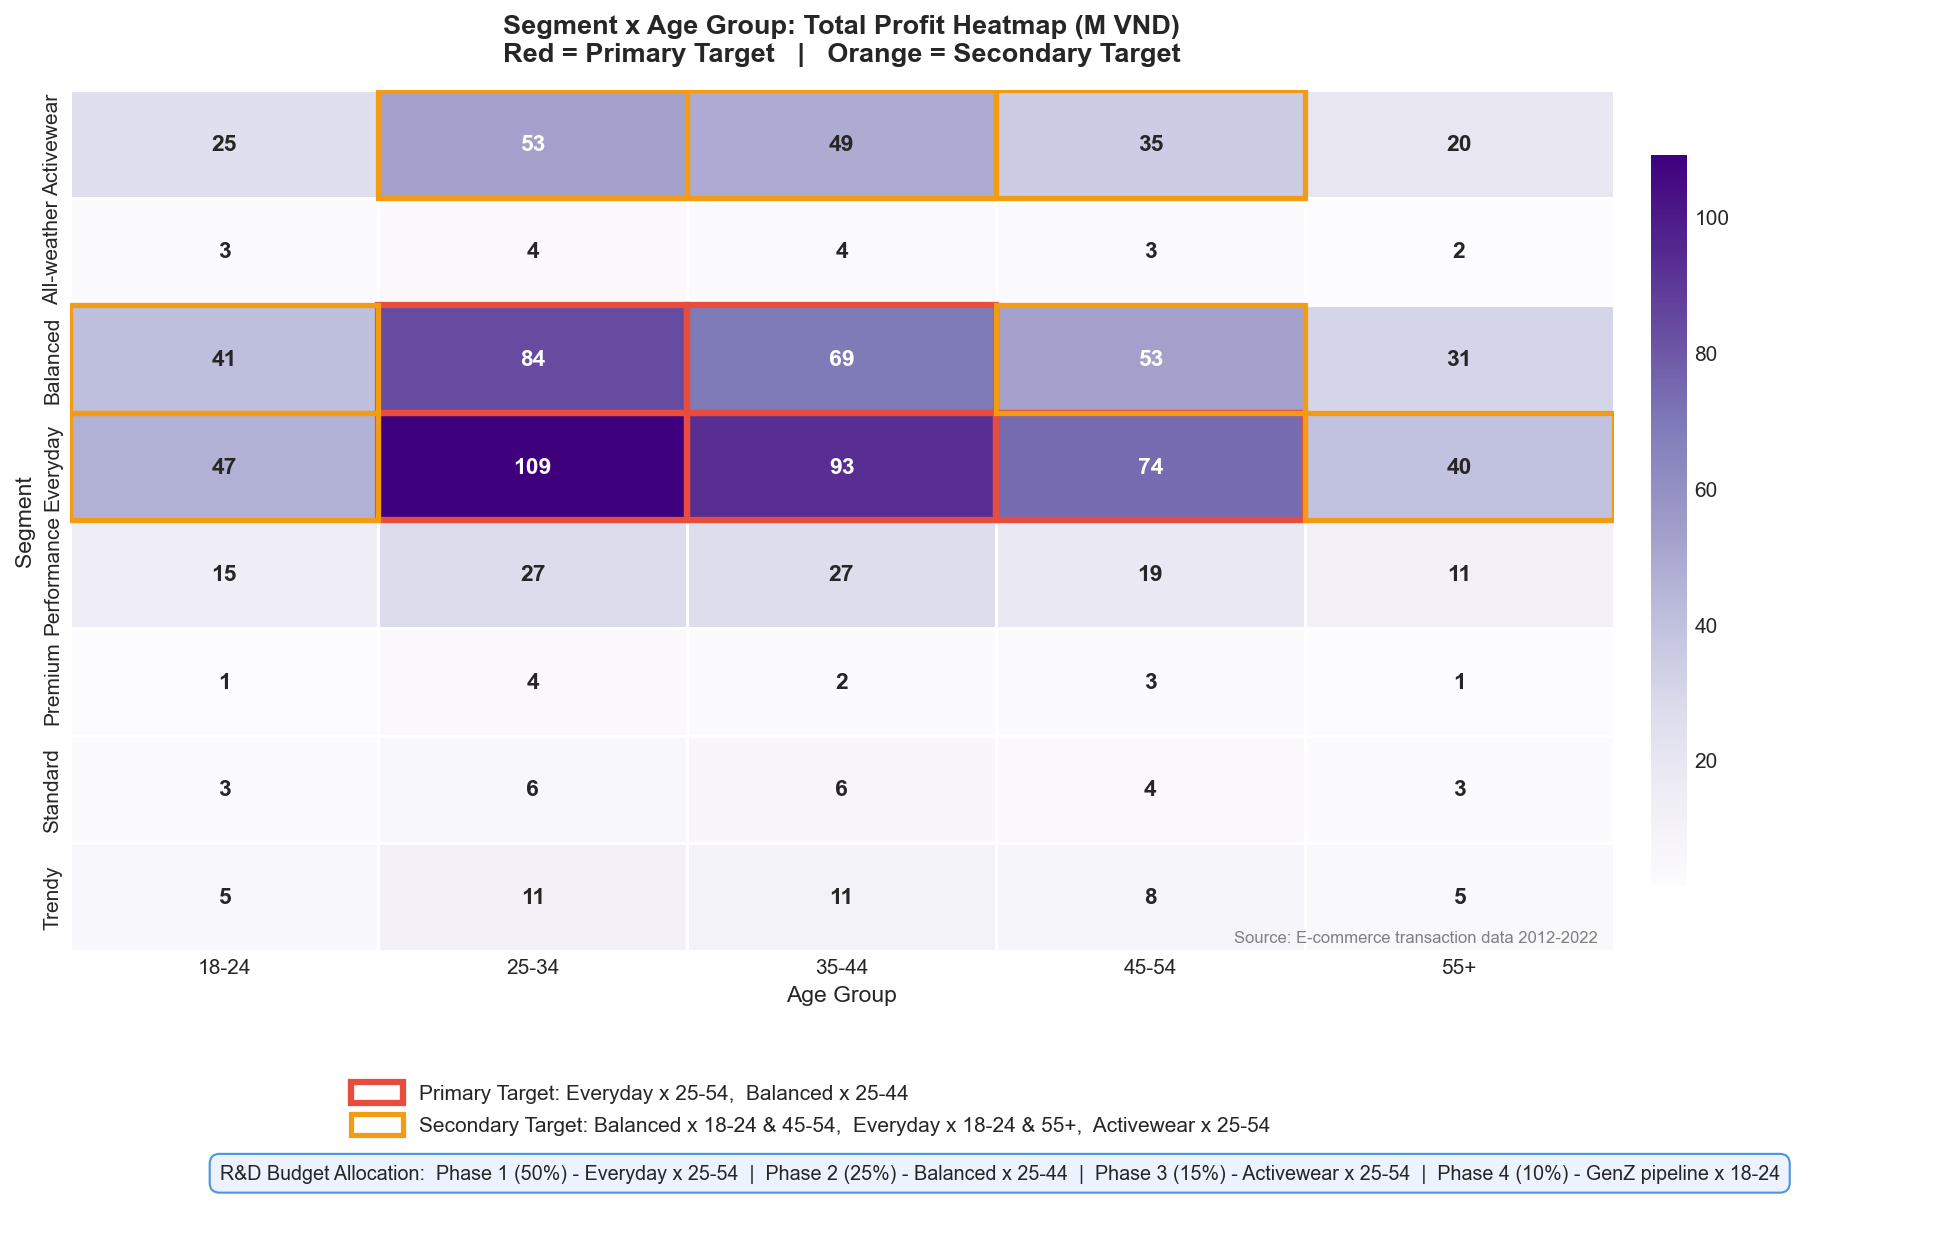
\includegraphics[width=1\textwidth]{datathon-2026-round-1/output/chart_17_segment_age_heatmap.png}
  \caption{Lợi nhuận theo Phân khúc và Nhóm tuổi}
  \label{fig:chart17}
\end{figure}

\begin{figure}[htbp]
  \centering
  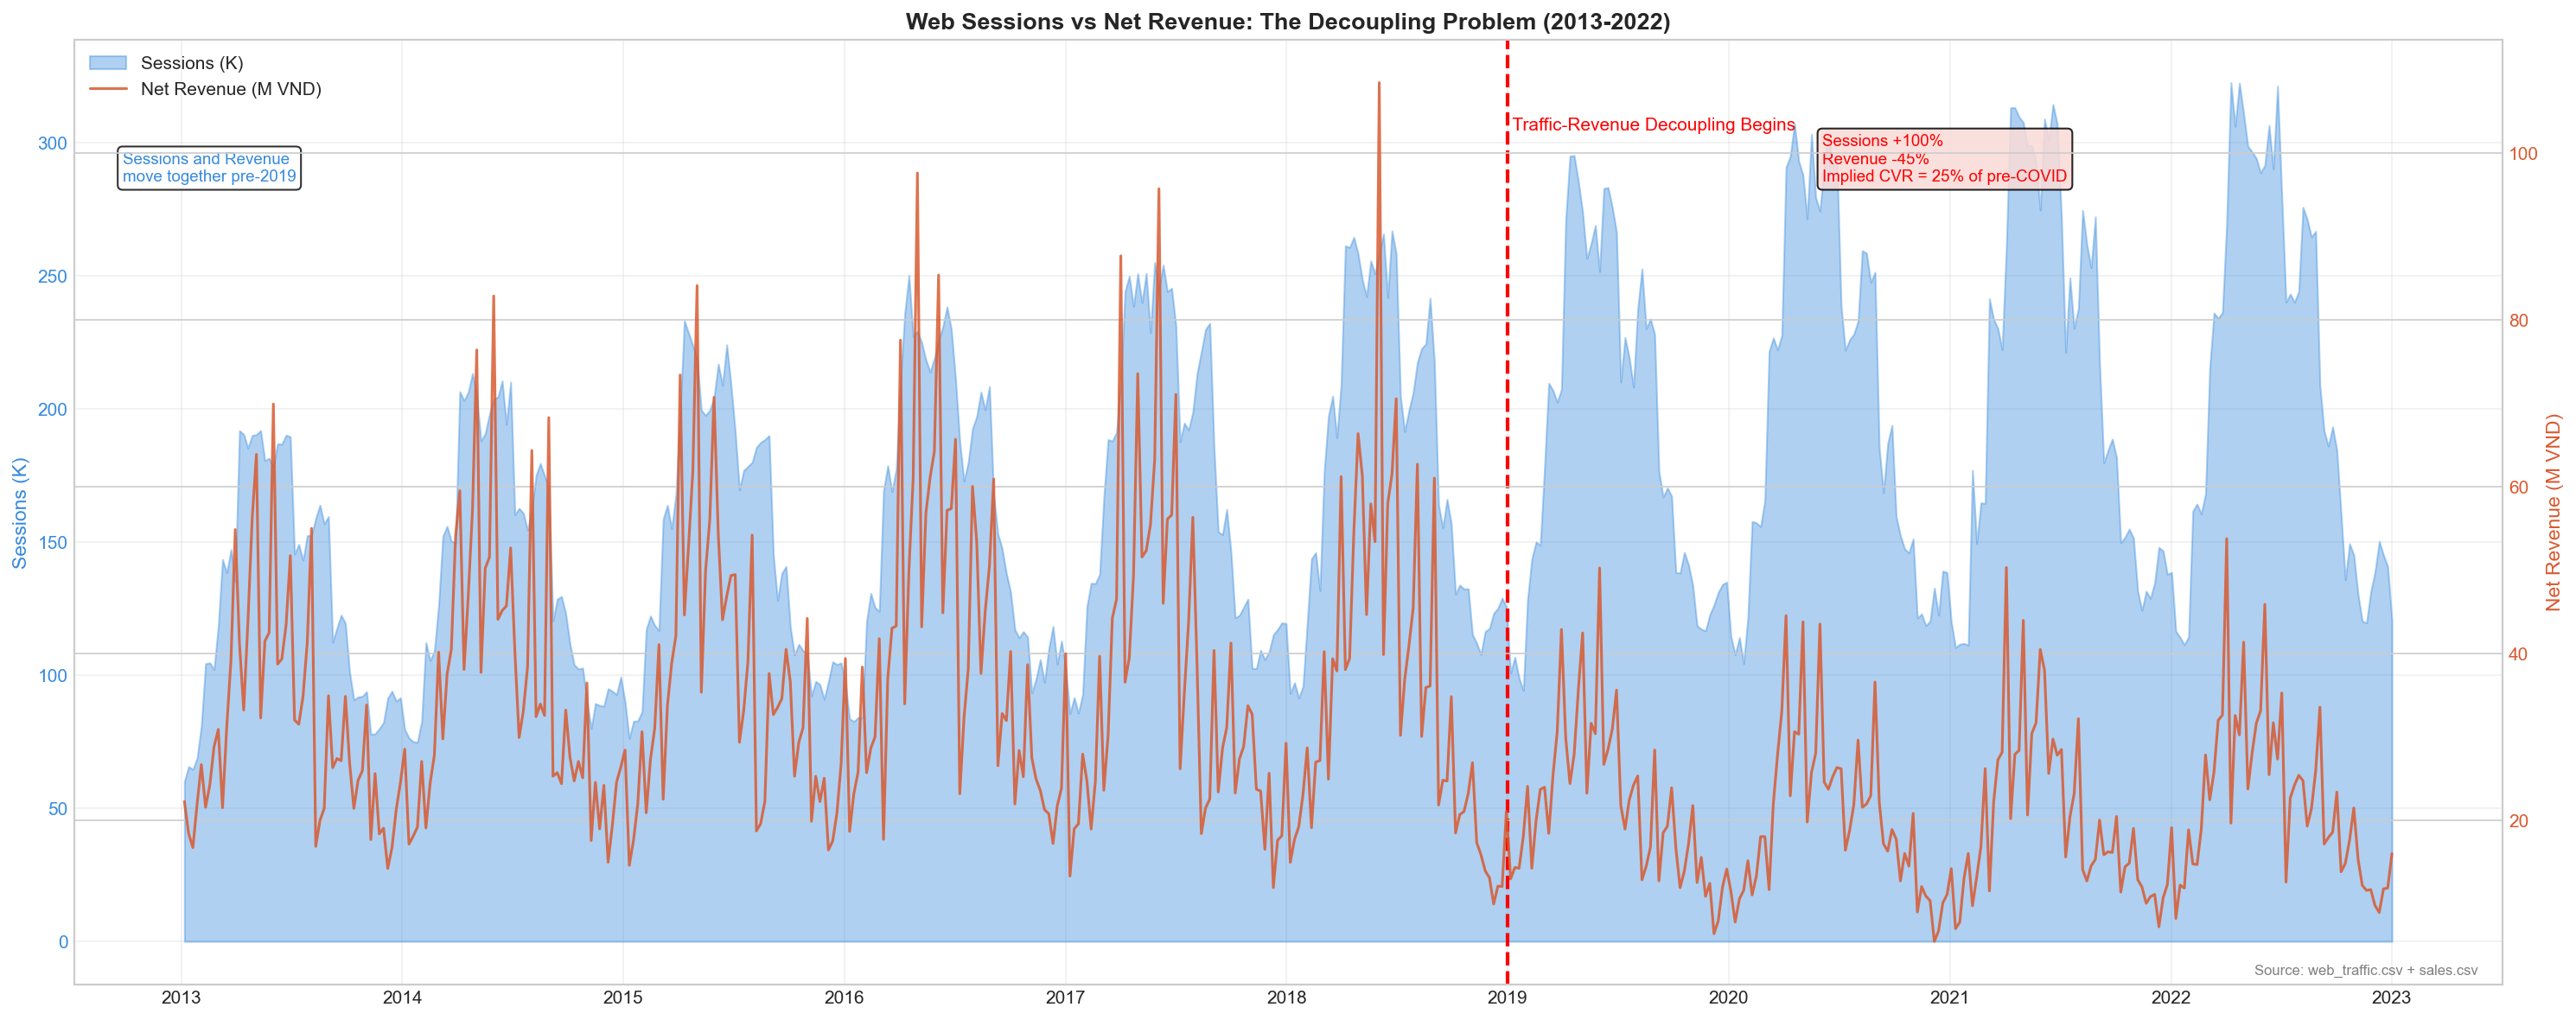
\includegraphics[width=1\textwidth]{datathon-2026-round-1/output/chart_14_sessions_revenue_decoupling.png}
  \caption{Nghịch lý Traffic \& Lợi nhuận ròng hậu COVID}
  \label{fig:chart14}
\end{figure}

\begin{figure}[htbp]
  \centering
  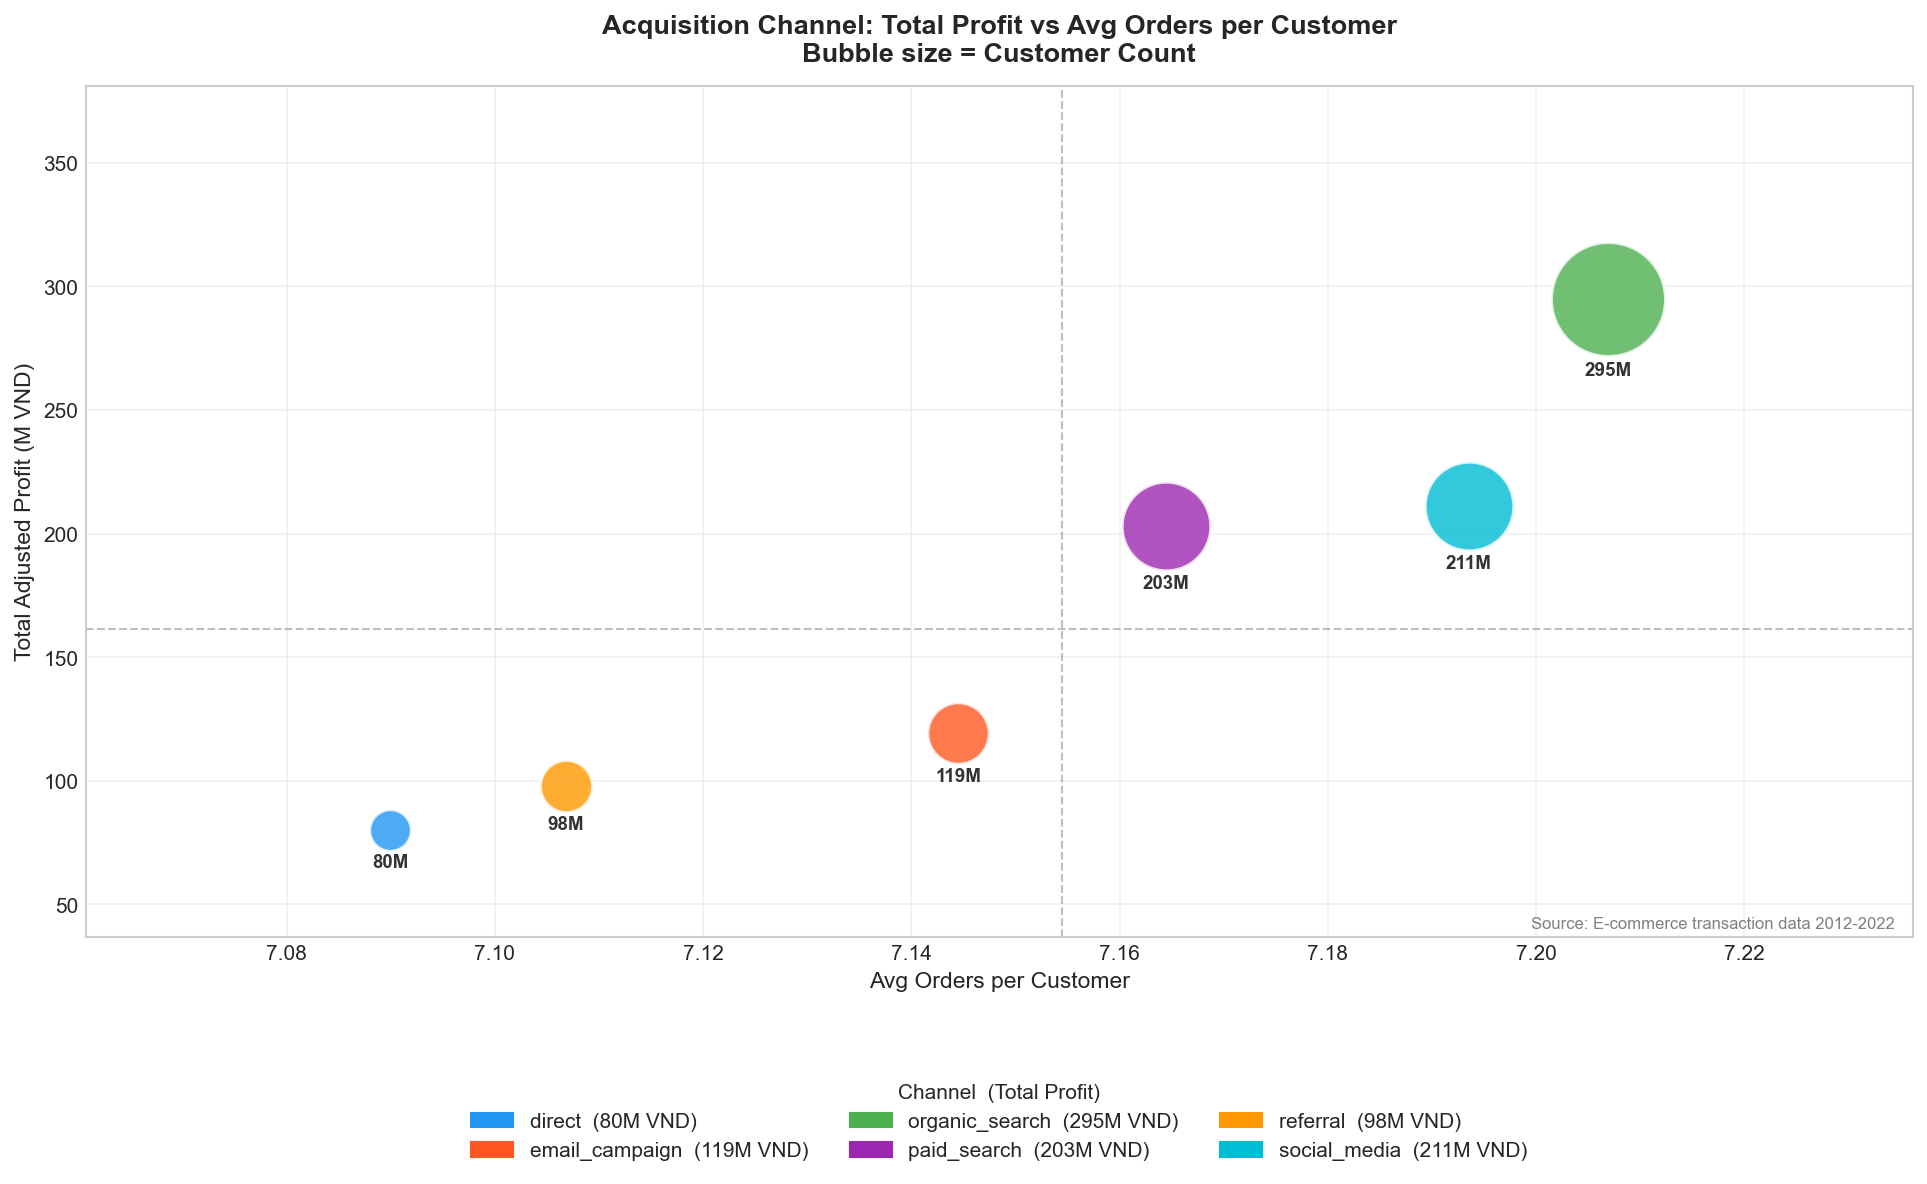
\includegraphics[width=1\textwidth]{datathon-2026-round-1/output/chart_07_channel_bubble.png}
  \caption{Lợi nhuận theo Kênh thu hút khách hàng}
  \label{fig:chart7}
\end{figure}

\begin{sidewaysfigure}[htbp]
  \centering
  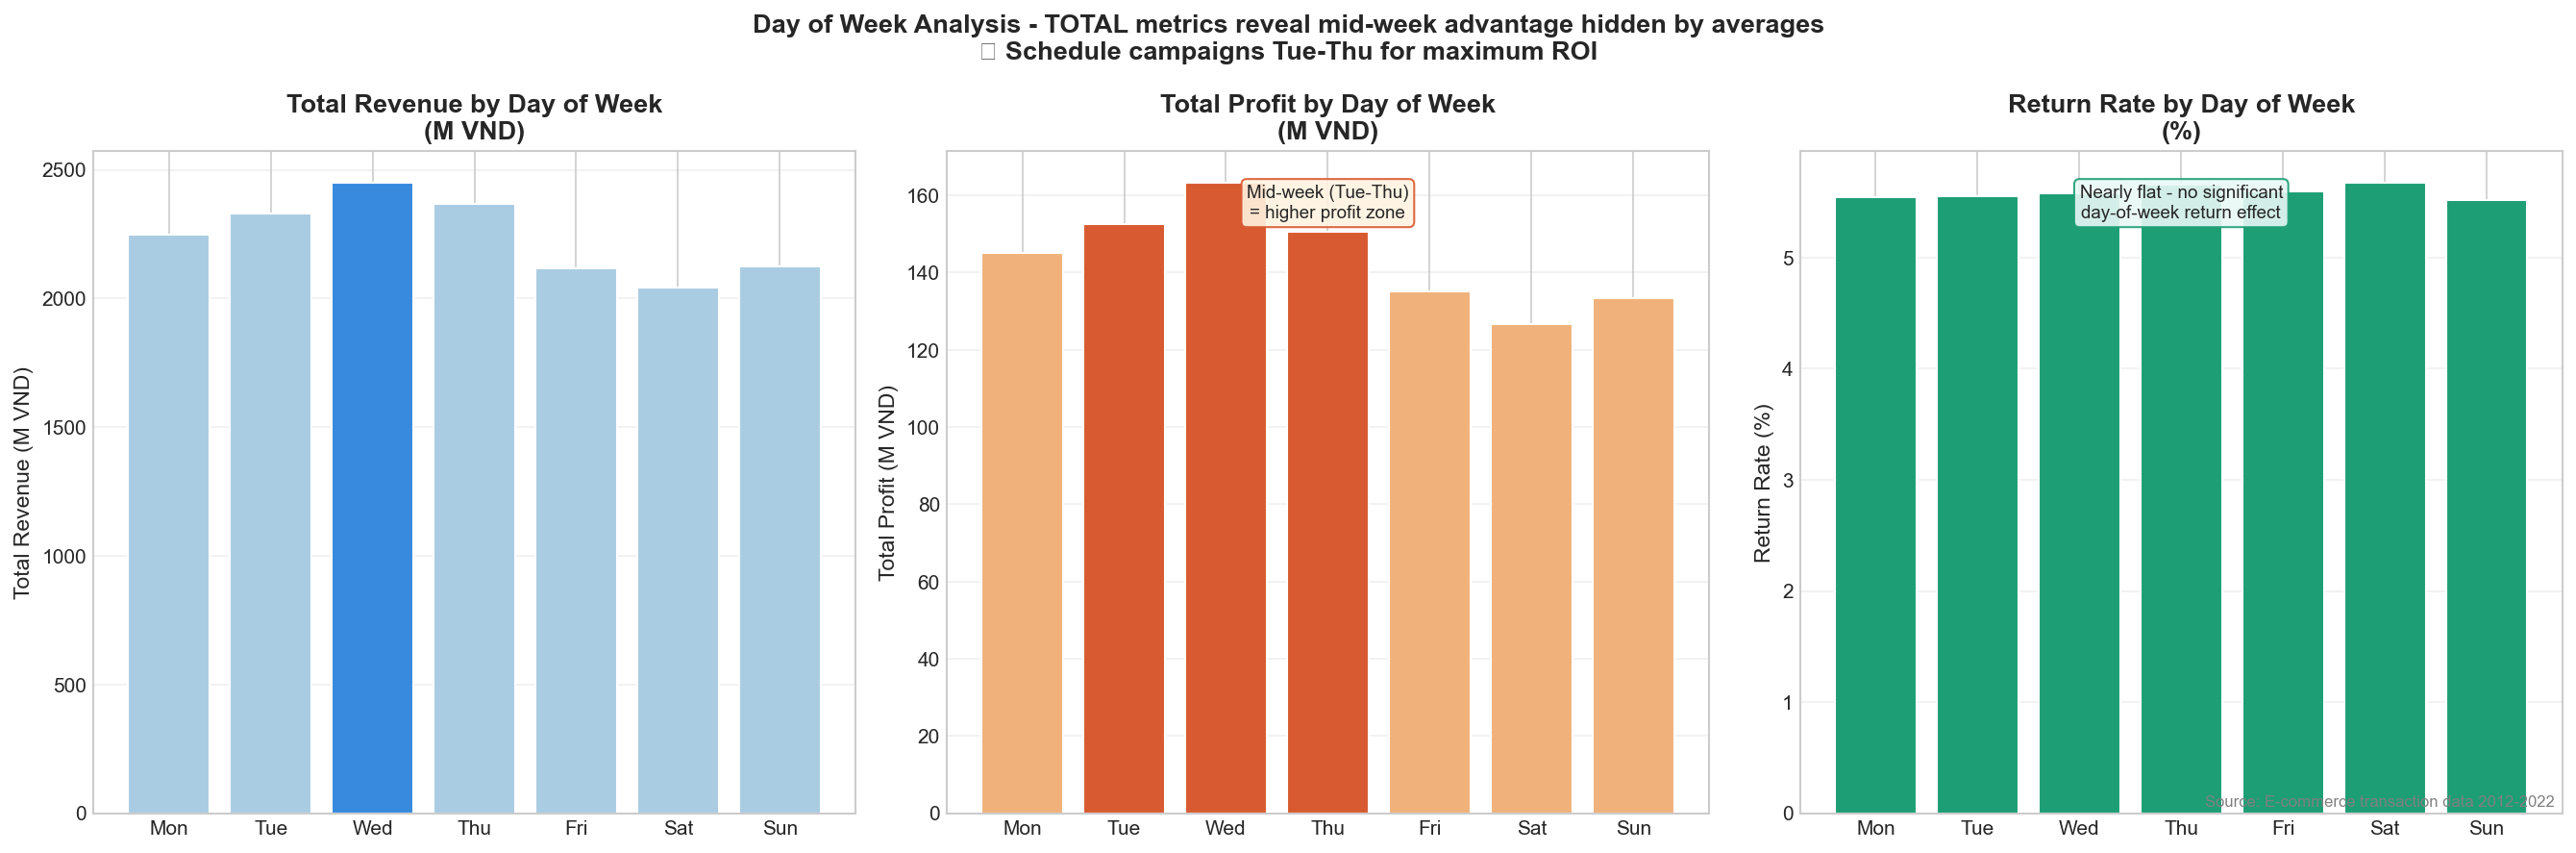
\includegraphics[width=0.95\textheight, height=0.9\textwidth, keepaspectratio]{datathon-2026-round-1/output/chart_09_day_of_week.png}
  \caption{Hành vi thanh toán theo ngày trong tuần}
  \label{fig:chart9}
\end{sidewaysfigure}

\begin{figure}[htbp]
  \centering
  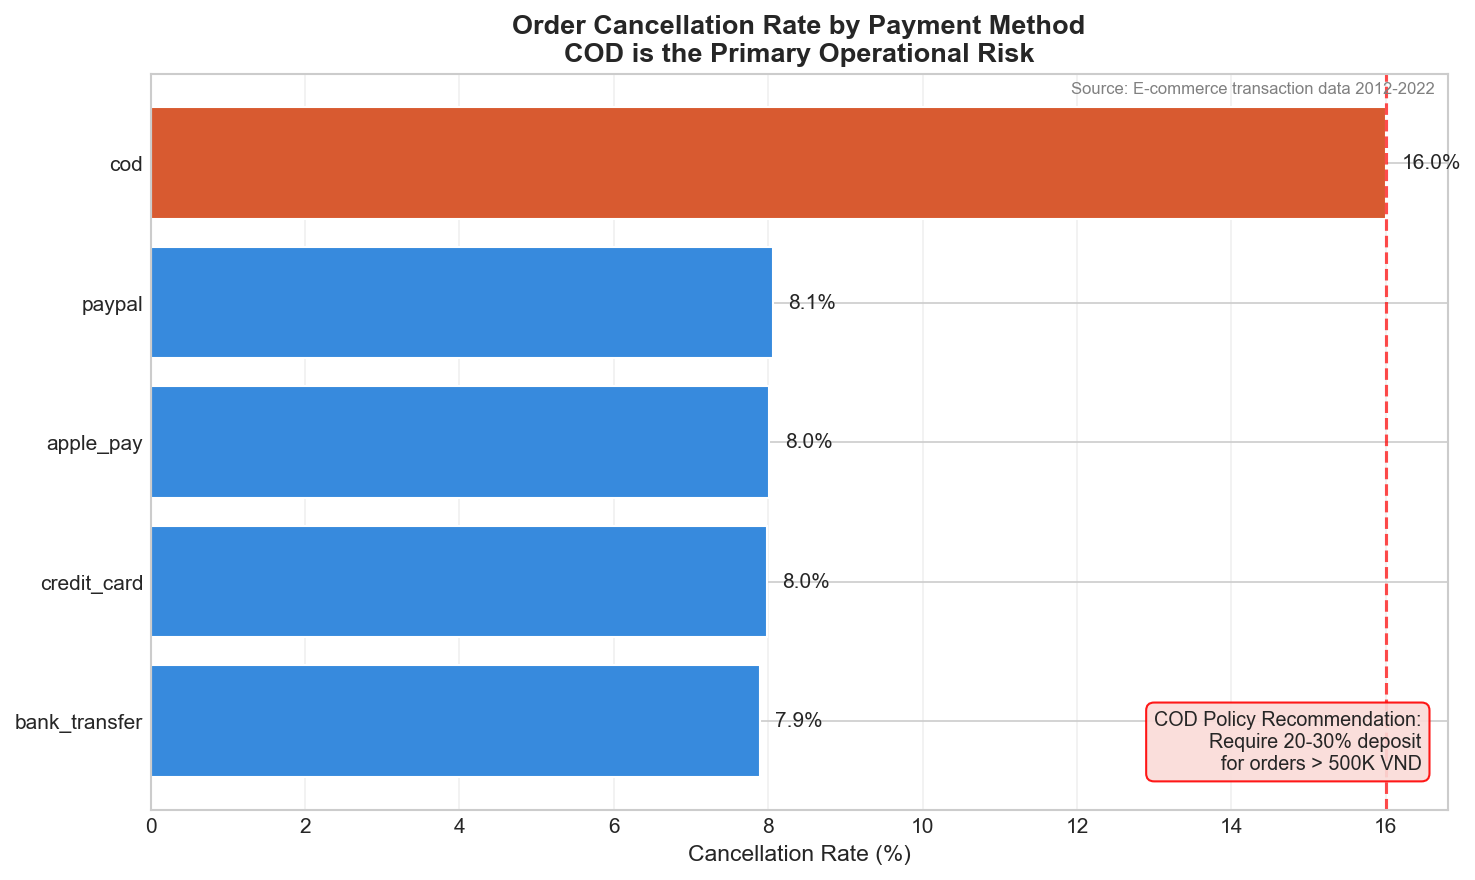
\includegraphics[width=1\textwidth]{datathon-2026-round-1/output/chart_10_cancellation_rate.png}
  \caption{Tỷ lệ huỷ đơn (COD vs phương thức khác)}
  \label{fig:chart10}
\end{figure}

\begin{figure}[htbp]
  \centering
  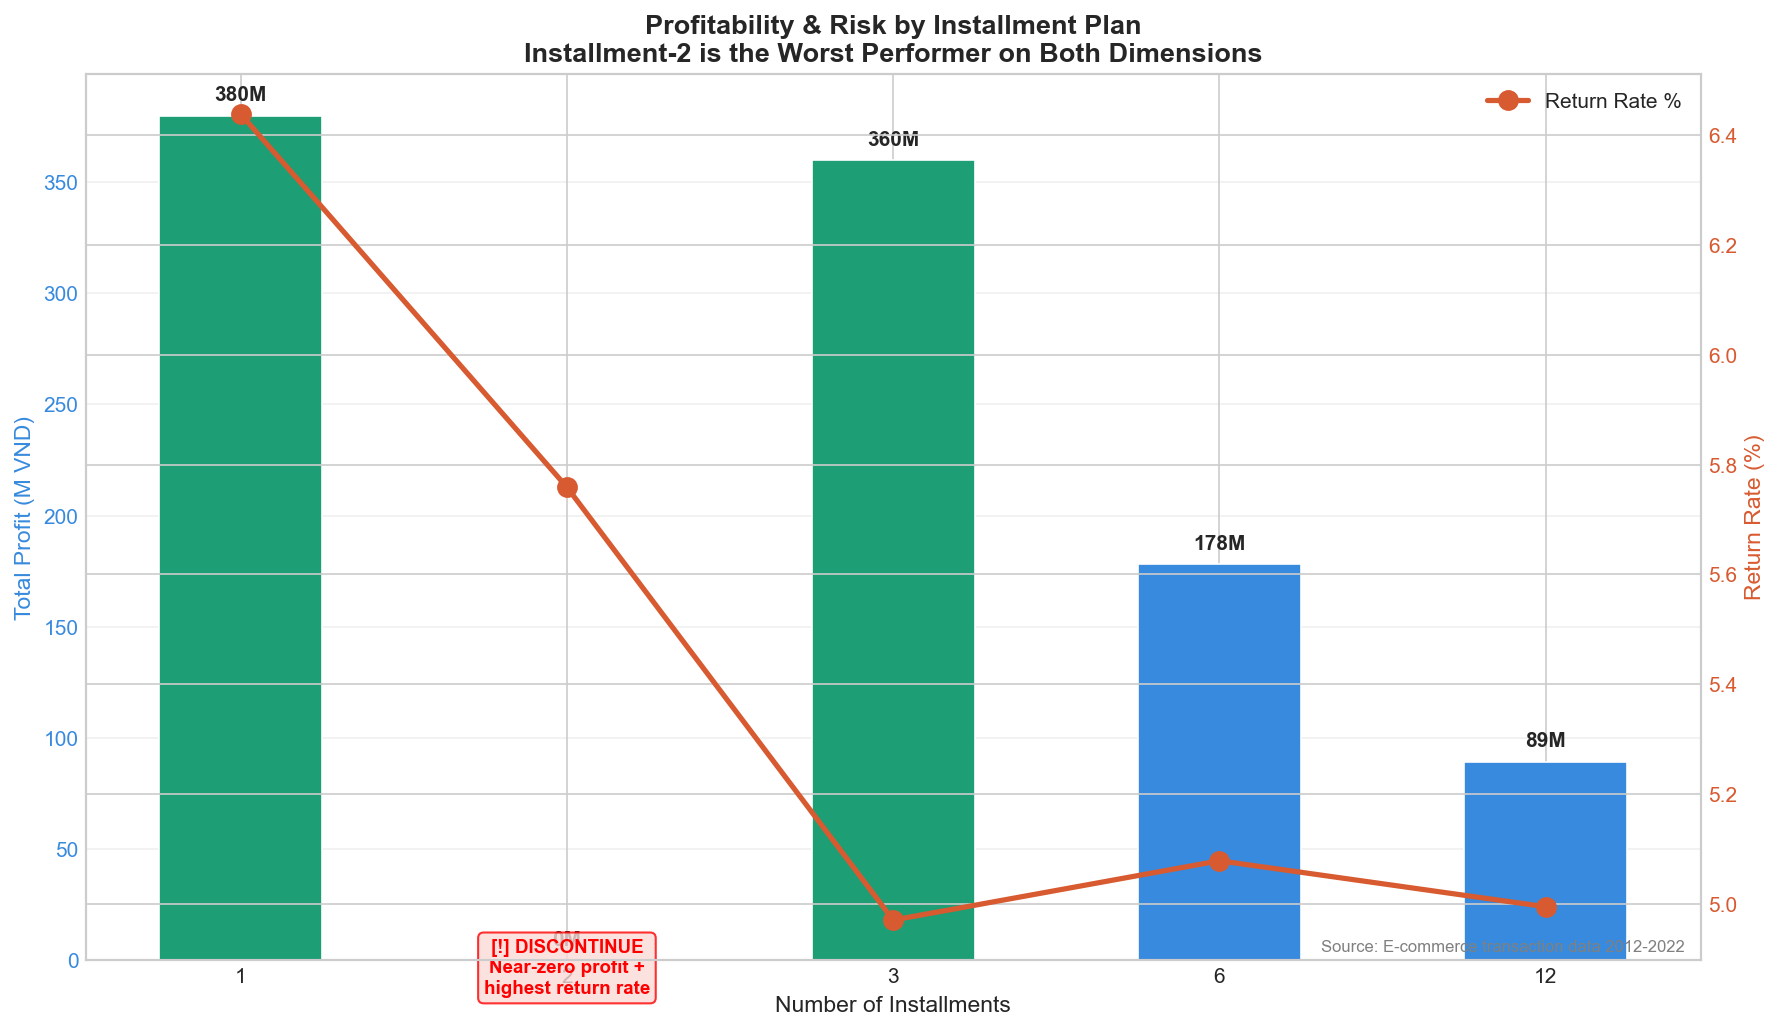
\includegraphics[width=1\textwidth]{datathon-2026-round-1/output/chart_11_installment_analysis.png}
  \caption{Phân tích độ rủi ro (Hoàn trả) theo gói trả góp}
  \label{fig:chart11}
\end{figure}

\begin{sidewaysfigure}[htbp]
  \centering
  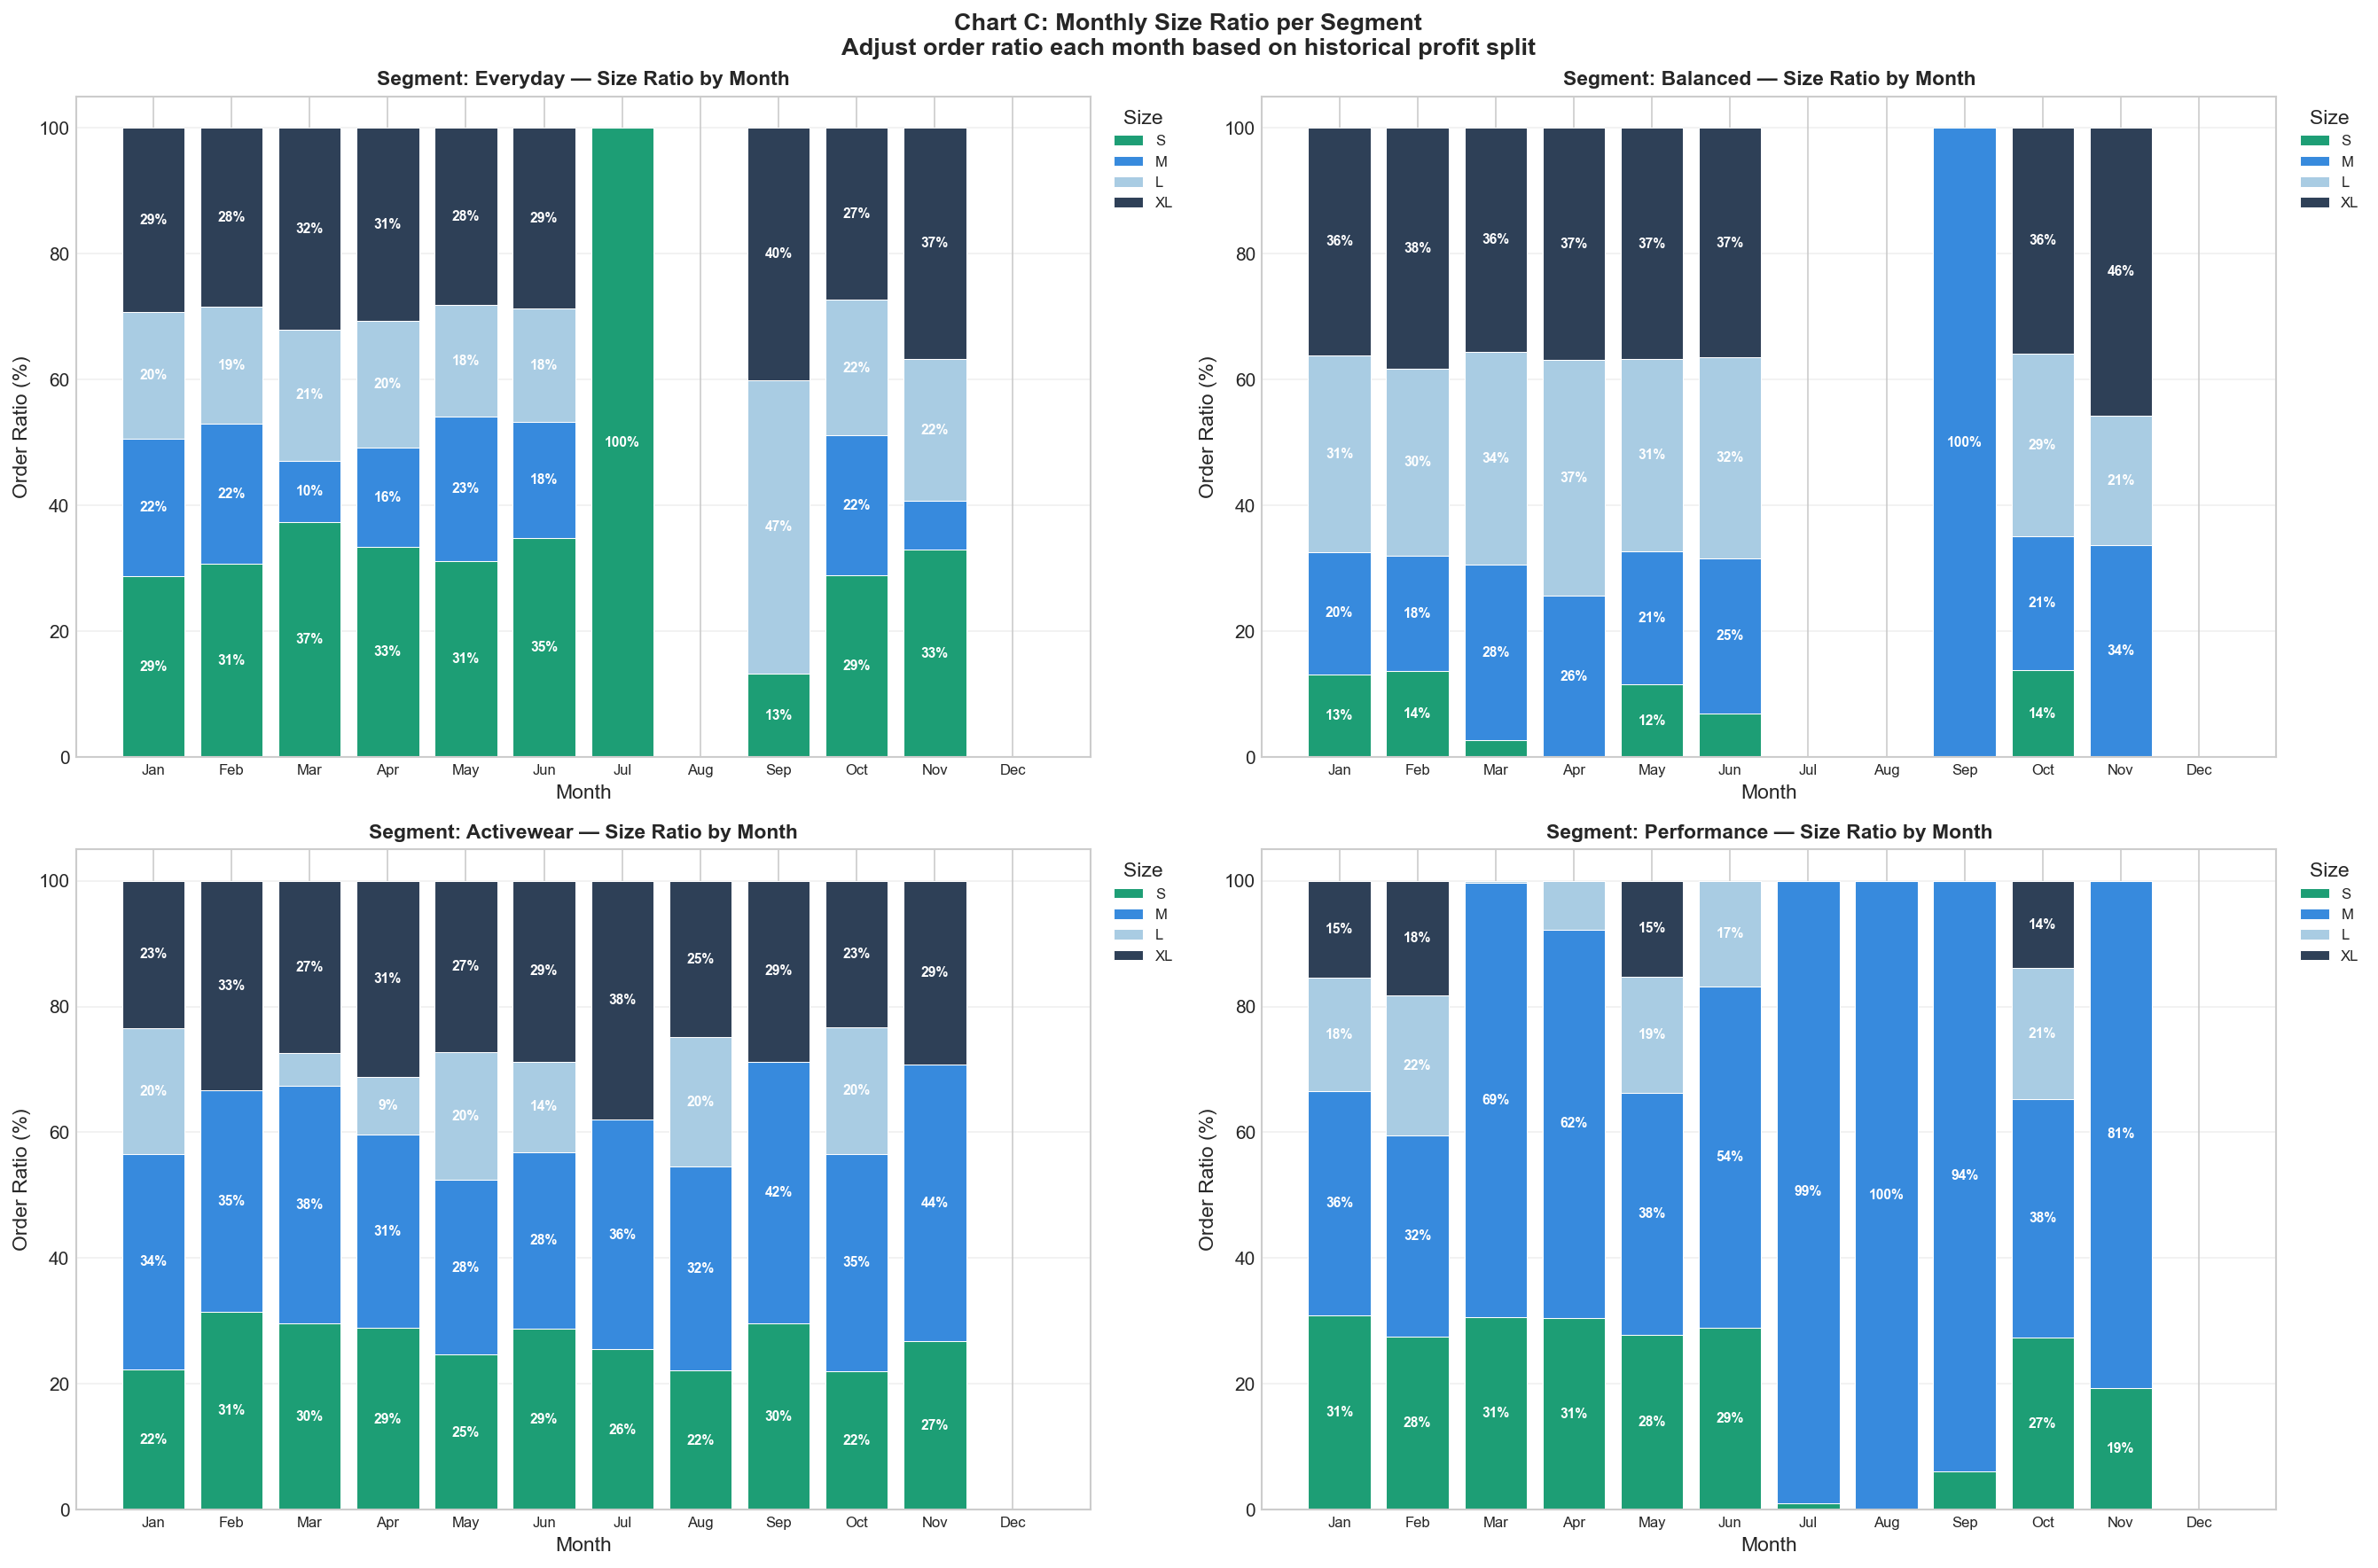
\includegraphics[width=0.95\textheight, height=0.9\textwidth, keepaspectratio]{datathon-2026-round-1/output/order_plan_C_size_by_month.png}
  \caption{Tỷ trọng tiêu thụ các Size theo Mùa vụ}
  \label{fig:chartC}
\end{sidewaysfigure}

\begin{figure}[htbp]
  \centering
  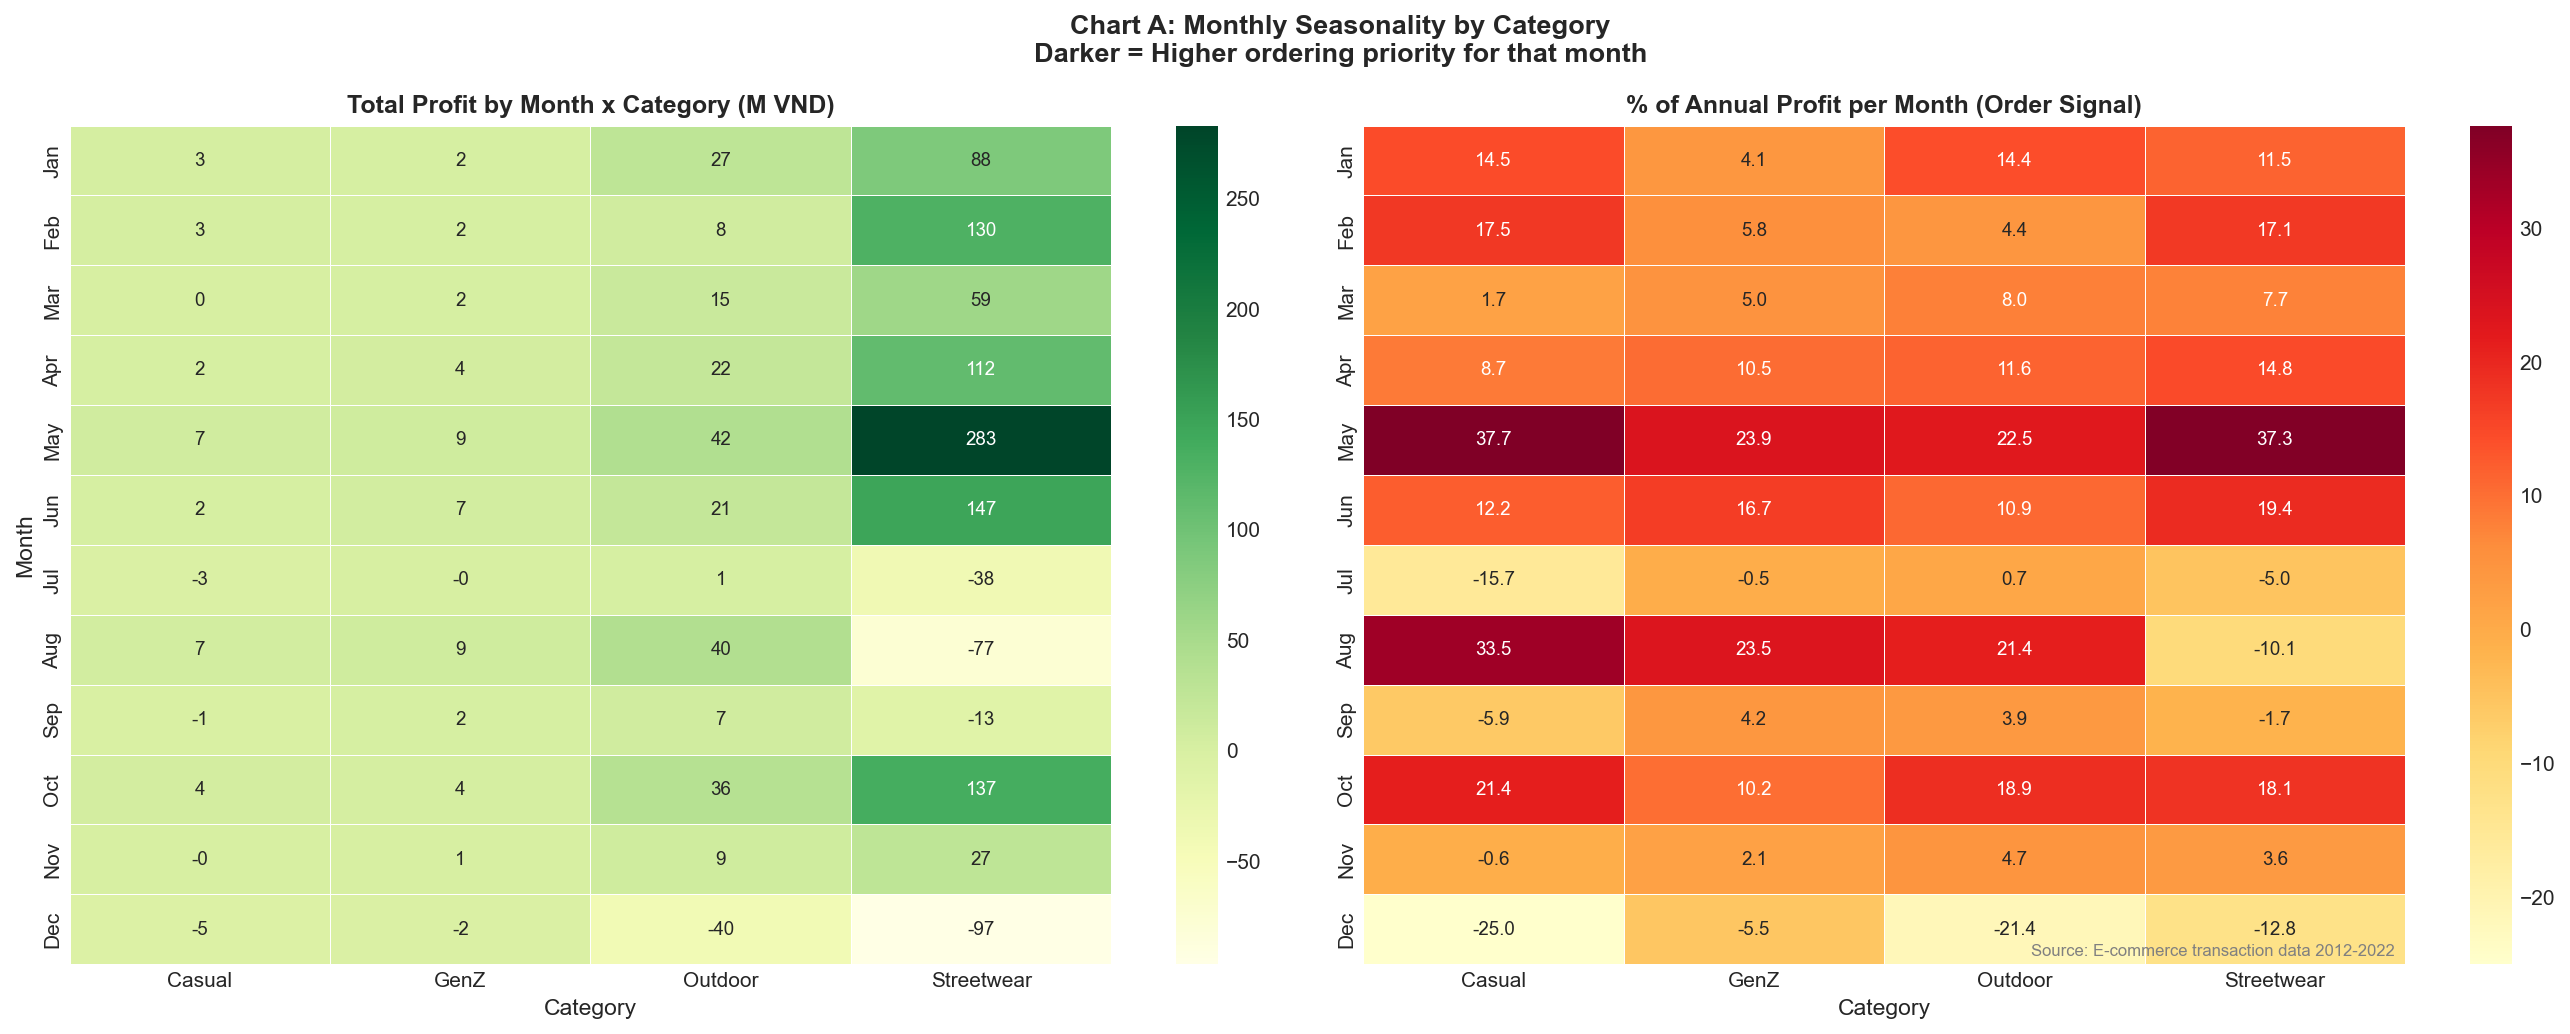
\includegraphics[width=1\textwidth, keepaspectratio]{datathon-2026-round-1/output/order_plan_A_month_category.png}
  \caption{Tính mùa vụ (Seasonality) theo Danh mục sản phẩm (Category)}
  \label{fig:chartA}
\end{figure}

\begin{figure}[htbp]
  \centering
  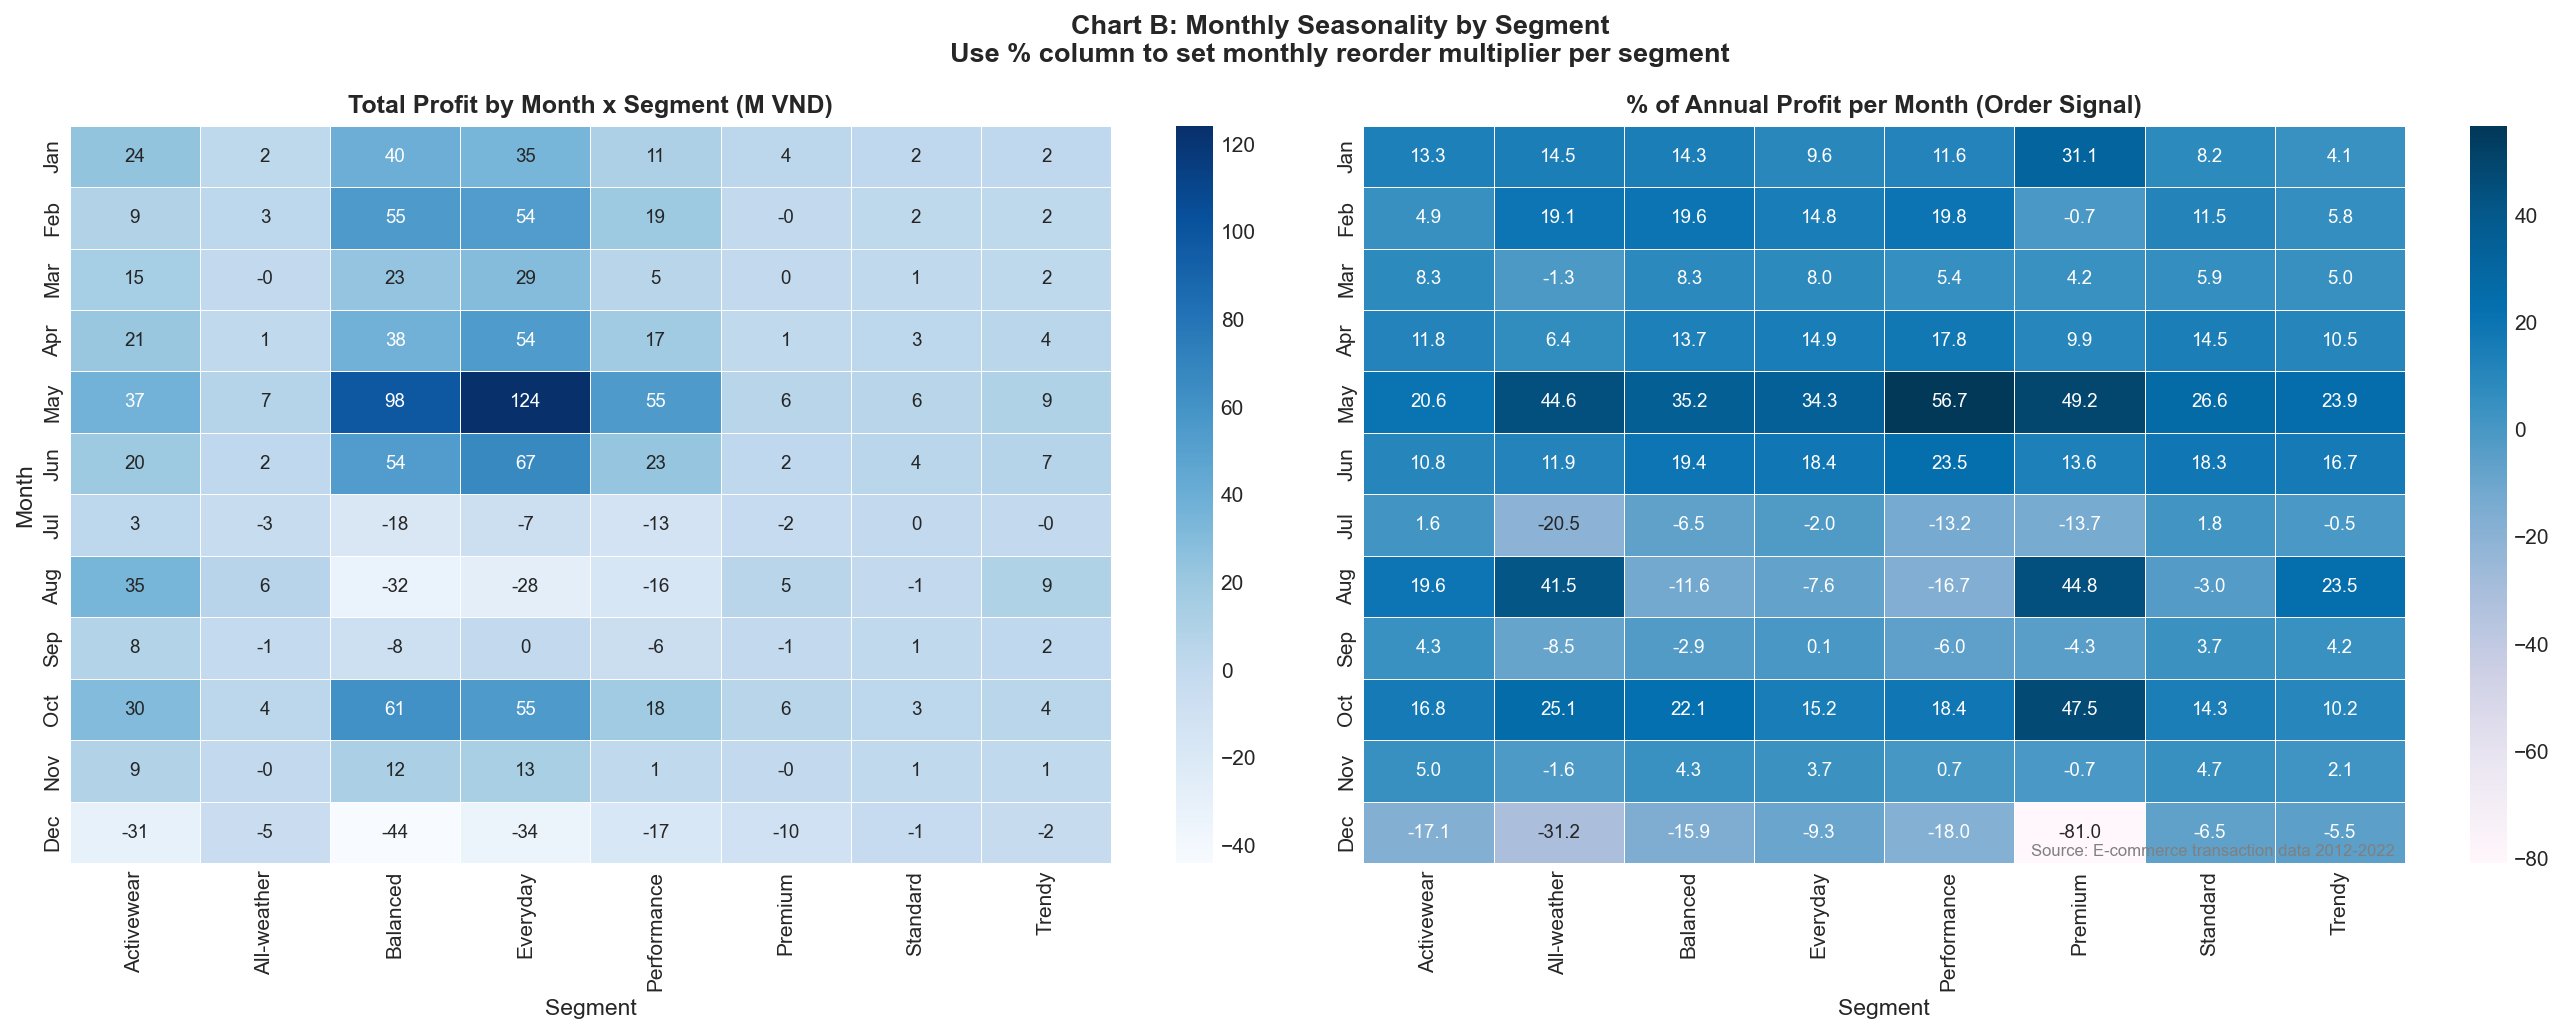
\includegraphics[width=1\textwidth, keepaspectratio]{datathon-2026-round-1/output/order_plan_B_month_segment.png}
  \caption{Tính mùa vụ (Seasonality) tỷ trọng Lợi nhuận theo Phân khúc (Segment)}
  \label{fig:chartB}
\end{figure}

\begin{figure}[htbp]
  \centering
  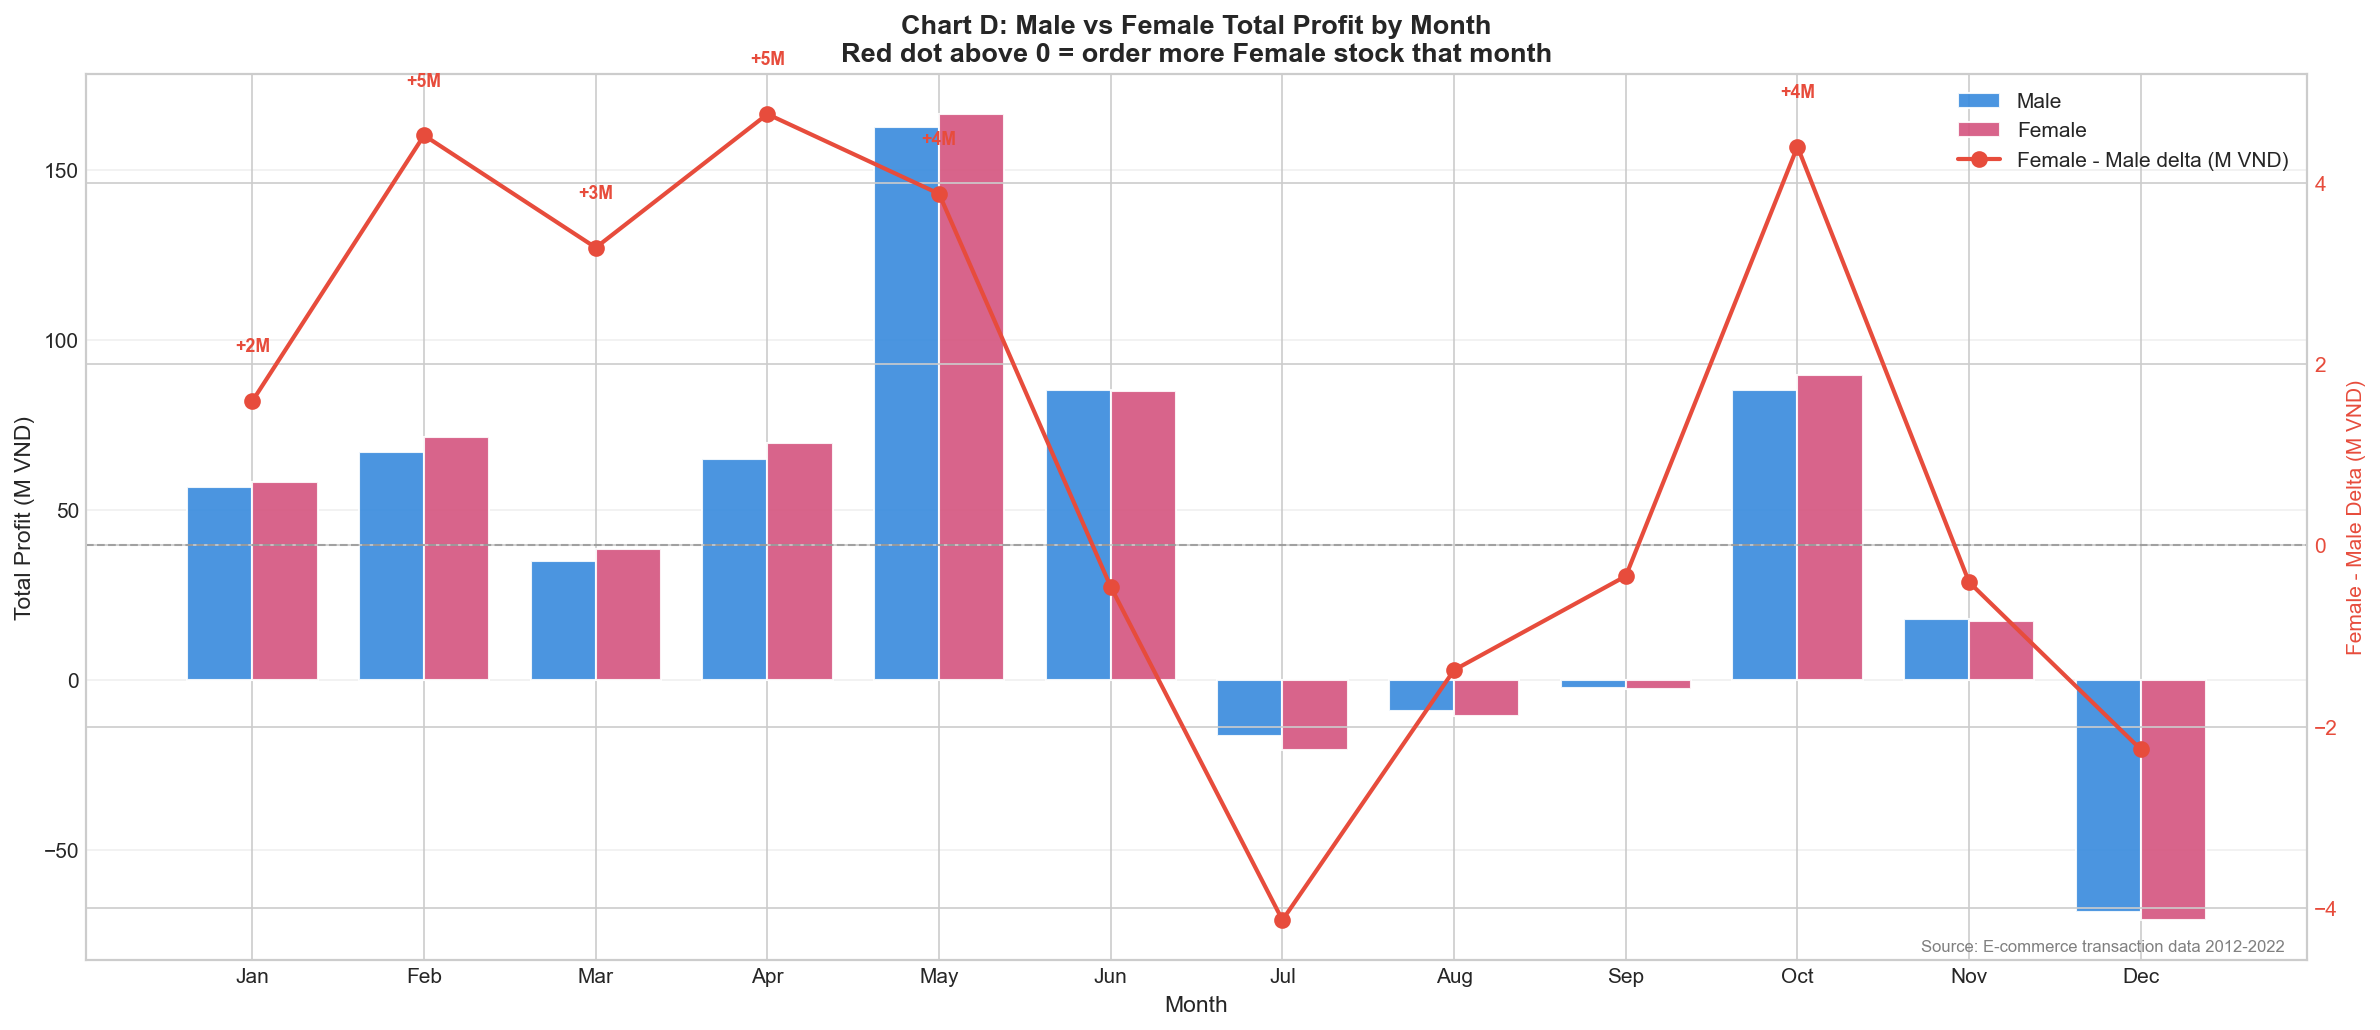
\includegraphics[width=1\textwidth, keepaspectratio]{datathon-2026-round-1/output/order_plan_D_gender_by_month.png}
  \caption{Tỷ trọng chi tiêu theo Giới tính từng tháng}
  \label{fig:chartD}
\end{figure}

\begin{sidewaysfigure}[htbp]
  \centering
  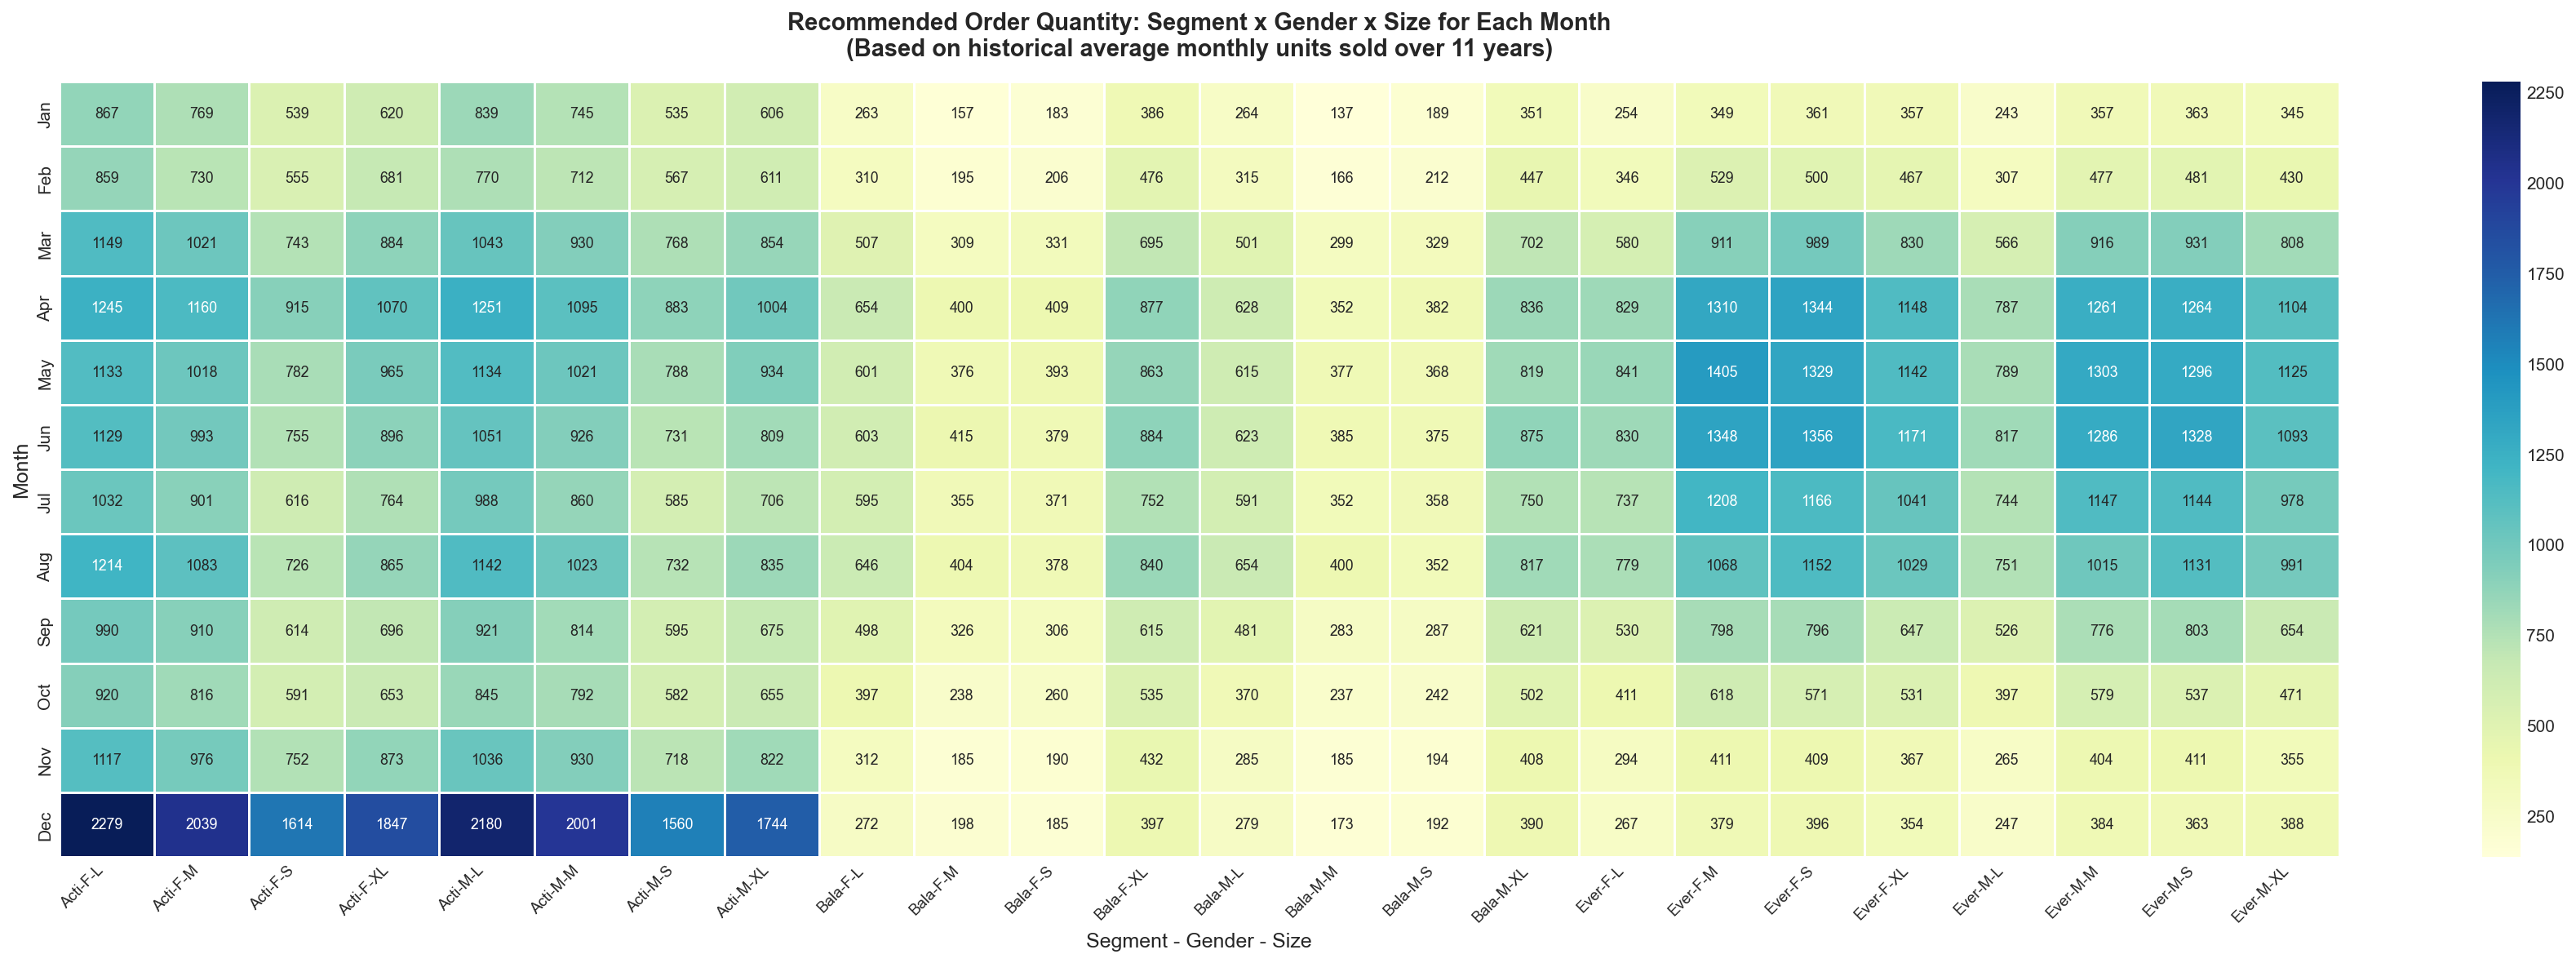
\includegraphics[width=0.95\textheight, height=0.9\textwidth, keepaspectratio]{datathon-2026-round-1/output/order_plan_F_detailed_quantity_matrix.png}
  \caption{Ma trận Cấu trúc Template Số lượng Sản xuất (Order Plan Quantity Matrix)}
  \label{fig:chartF}
\end{sidewaysfigure}

\begin{sidewaysfigure}[htbp]
  \centering
  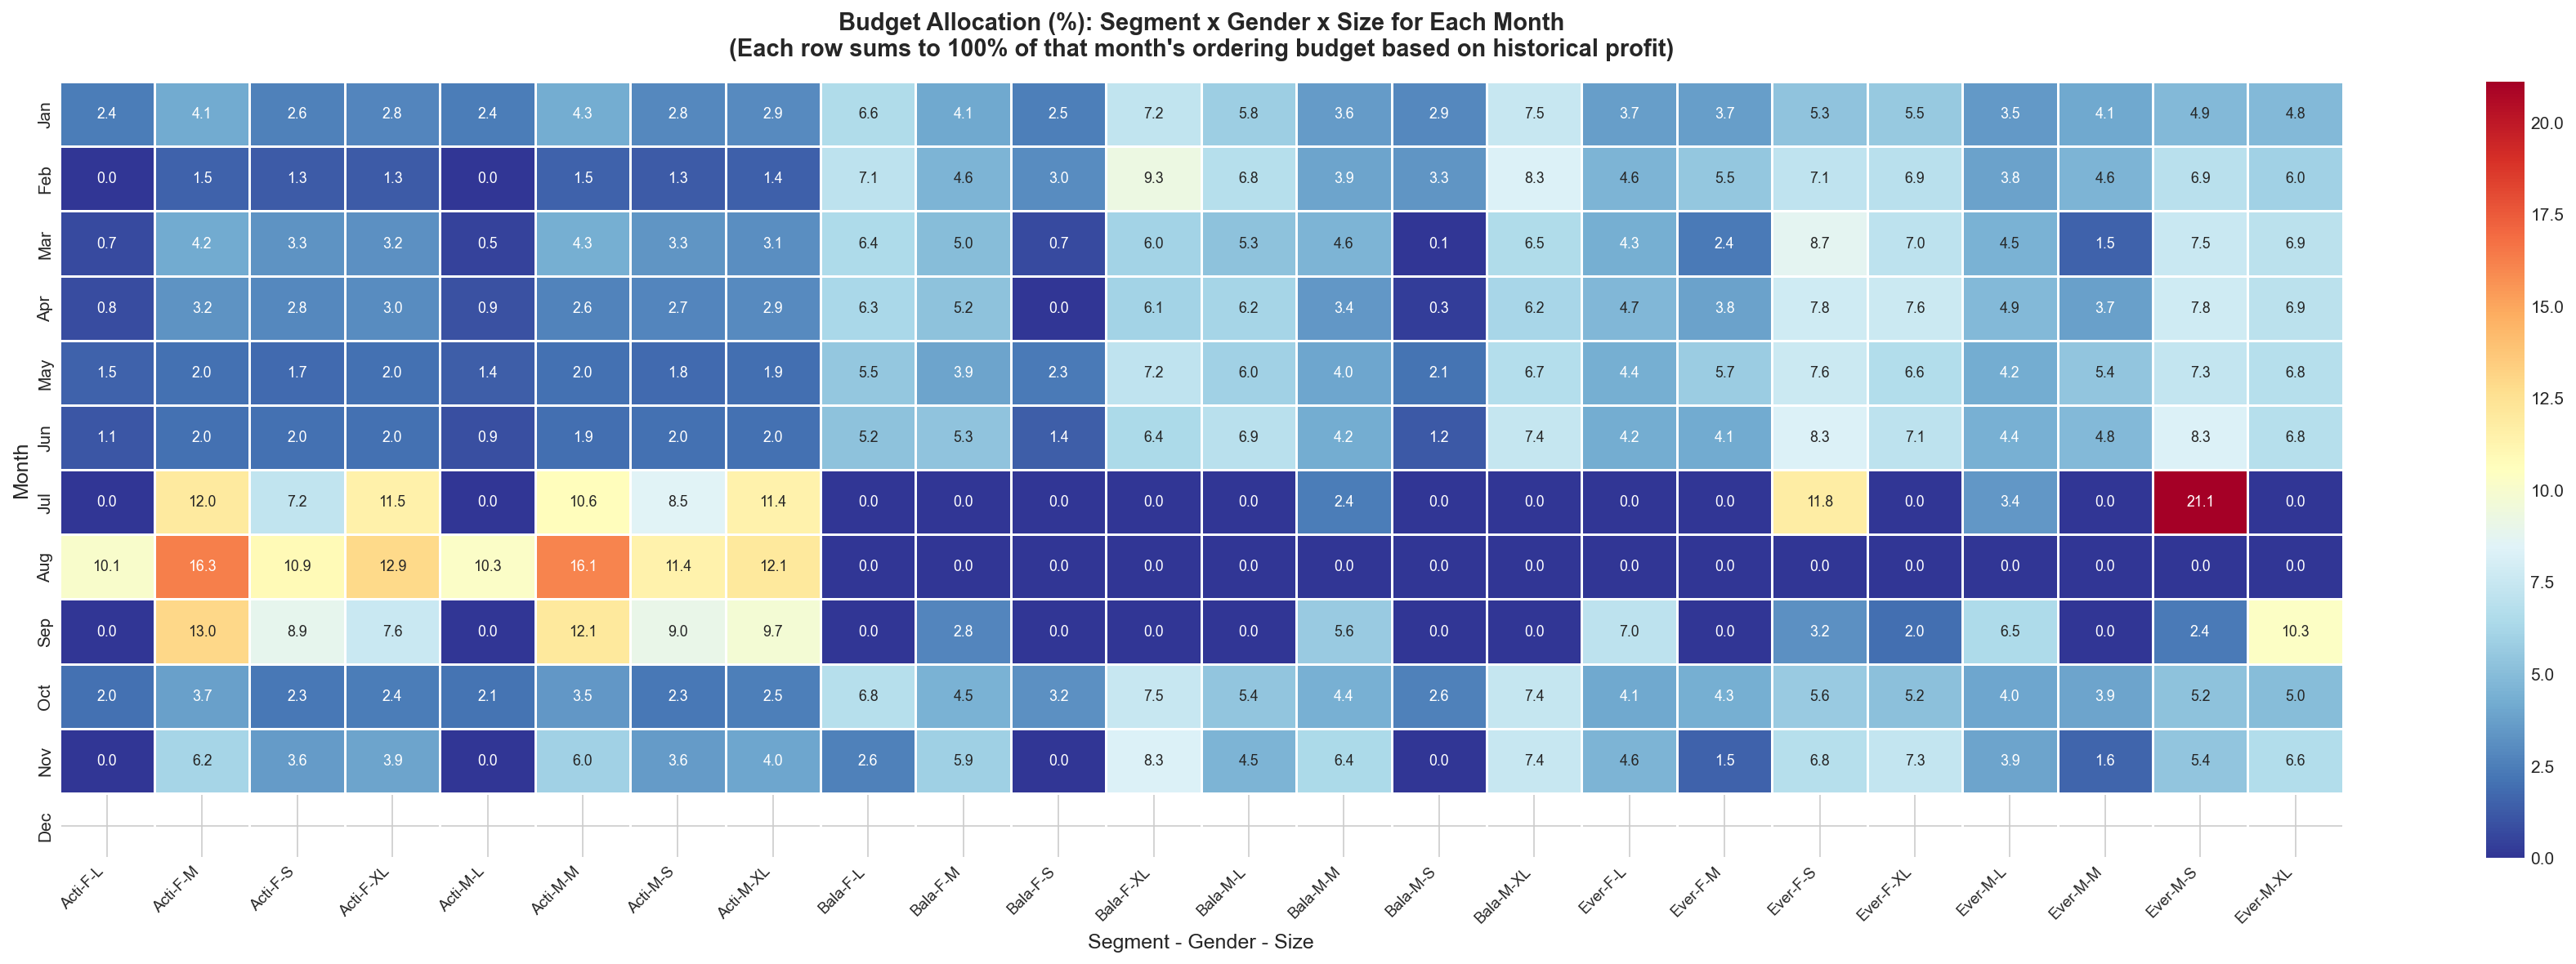
\includegraphics[width=0.95\textheight, height=0.9\textwidth, keepaspectratio]{datathon-2026-round-1/output/order_plan_G_detailed_profit_matrix.png}
  \caption{Ma trận Cấu trúc Template Kế hoạch Lợi nhuận (Order Plan Profit Matrix)}
  \label{fig:chartG}
\end{sidewaysfigure}

\clearpage
\section{Github Repository}
\textbf{Link:} \url{https://github.com/trmuba2502/VinUni_Datathon_4Chickens} \\
(Kho mã nguồn thiết lập môi trường, feature engineering báo cáo cho \texttt{05\_forecast\_final.py}, file submission \texttt{.csv} và scripts trực quan biểu đồ).

\end{document}